%!TEX root = Manuscript.tex

\chapter{Precise matching}
\label{chap:intro}
\minitoc

\section{Introduction}
\subsection{Motivation}
\subsection{Contribution}
check SIFT scale and rotation\\
\textit{one-to-one tiling scheme}\\
3D ransac?

\section{Methodology}
To compute precise {inter-epoch} matches, we perform matching on original RGB images {under the guidance of co-registered orientations and DSMs}. {It consists of extracting tentative inter-epoch matches, followed by a 3D-RANSAC filter and a cross correlation stage to remove outliers.} The workflow is displayed in Figure~\ref{WorkflowPatch}(a).
\par
We choose matching RGB images for precise matching instead of DSMs, as the DSMs are noisy due to low radiometric quality of the images. In Appendix~\ref{chap:appendix4} we compared the matching results on RGB images and DSMs over the same area. It demonstrated that there are more numerous but less accurate matches found in DSMs. As the goal of precise matching is to recover accurate matches, the RGB images are more suitable than DSMs.\\

\begin{figure*}[htbp]
	\begin{center}
		\subfigure[Workflow]{
			\begin{minipage}[t]{1\linewidth}
				\centering
				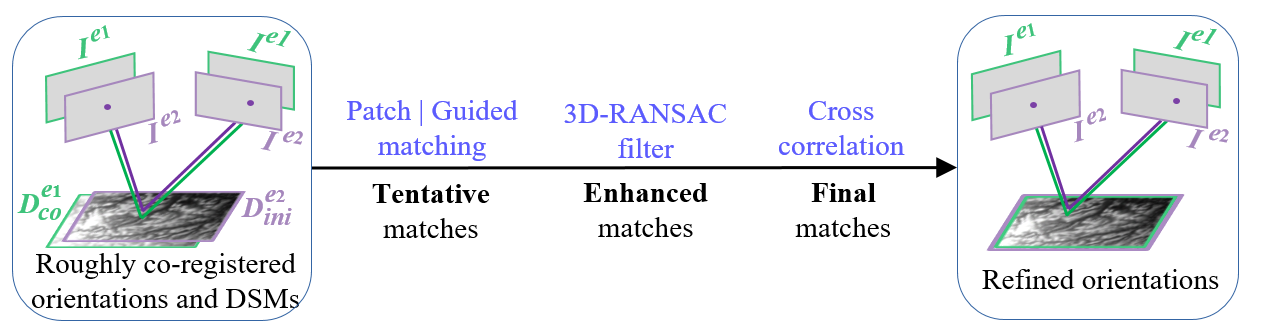
\includegraphics[width=1\columnwidth]{images/Chapitre4/precisematching.png}
			\end{minipage}%
		}
		\subfigure[Patch matching]{
			\begin{minipage}[t]{0.35\linewidth}
				\centering
				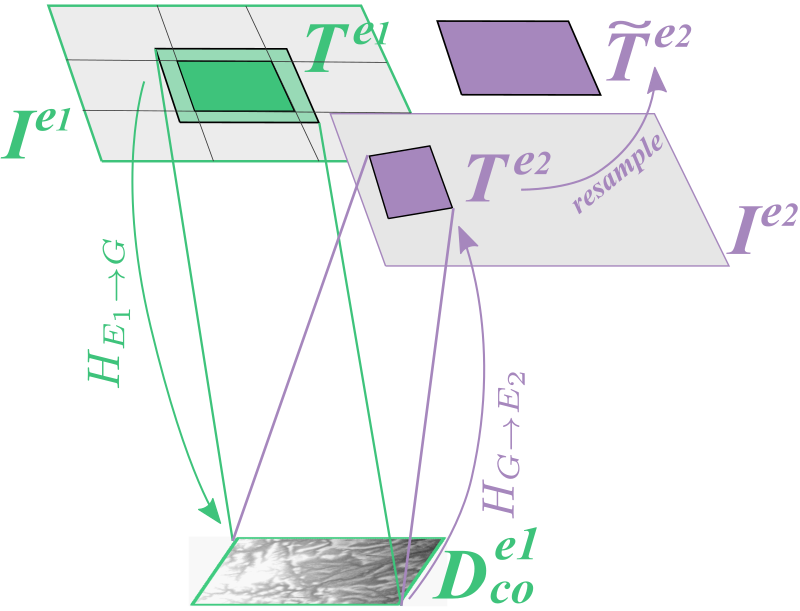
\includegraphics[width=4.5cm]{images/Chapitre4/patchmatching.png}
			\end{minipage}%
		}
		\subfigure[Buffer zone of tiles]{
			\begin{minipage}[t]{0.25\linewidth}
				\centering
				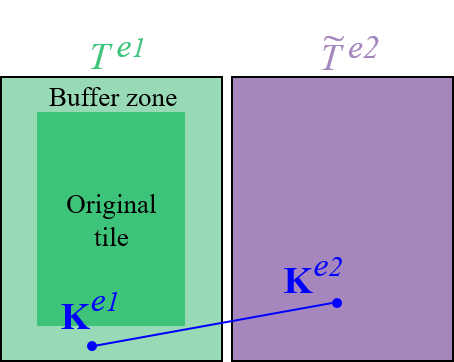
\includegraphics[width=3.8cm]{images/Chapitre4/tilingScheme.png}
			\end{minipage}%
		}
		\subfigure[Guided matching]{
			\begin{minipage}[t]{0.35\linewidth}
				\centering
				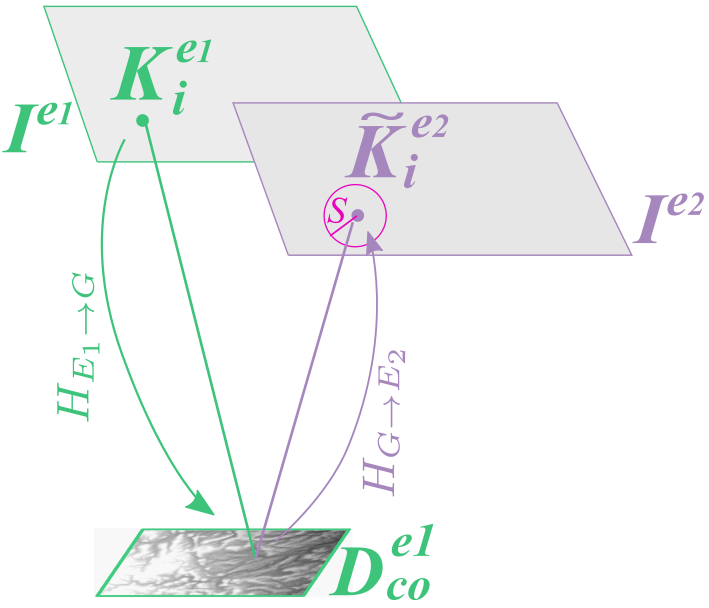
\includegraphics[width=4.5cm]{images/Chapitre4/guidedmatching.png}
			\end{minipage}%
		}
		\caption{(a) Workflow of precise matching. It is carried out by performing patch or guided matching to obtain tentative matches, followed by 3D-RANSAC filter and cross correlation, giving rise to final matches. (b) and (d) illustrate toy-examples of the patch matching and guided matching, respectively. (c) displays the feature correspondences where $\mathbf{K}^{e_1}$ exceeds the original tile size (dark green area) and therefore will be abandoned.}
		\label{WorkflowPatch}
	\end{center}
\end{figure*}

\subsection{Get tentative matches}\label{patch matching}
We offer two alternatives to recover tentative matches: patch or guided matching. {The former has better overall} performance while the latter is more efficient in terms of the use of memory and CPU resources.\\
\subsubsection{Patch matching for learned features}
{{It} is based on \textit{one-to-one tiling scheme}} {(not to confuse with the \textit{one-to-many tiling scheme} presented in the \textit{rough co-registration}), as shown in Figure~\ref{WorkflowPatch}(b) and detailed below}:
\begin{enumerate}
	%\item Crop the master RGB image $I^{e_1}$ into M tiles ($T^{e_1}$) of certain size (640$\times$480 pixels in our experiments), with a buffer zone (64 pixels in the width and 48 pixels in the height in our experiments) overlapped with each other;
	\item Crop the master RGB image $I^{e_1}$ into M original tiles of certain size, and expand them with a buffer zone (as shown in Figure~\ref{WorkflowPatch}(c)), giving rise to M buffered tiles ($T^{e_1}$);
	\item Project each buffered tile $T^{e_1}$ onto the DSM $D_{co}^{e_1}$ and backproject to secondary RGB image $I^{e_2}$ to find the corresponding tile $T^{e_2}$;
	\item Resample $T^{e_2}$ to $\widetilde{T}^{e_2}$, so that the tile pair $P({T^{e_1},\widetilde{T}^{e_2}})$ is free from differences of rotation, scale and extent;
	\item Apply SuperGlue on tile pair $P({T^{e_1},\widetilde{T}^{e_2}})$ to find matches $M({\mathbf{K}^{e_1},\mathbf{K}^{e_2}})$ ($\mathbf{K}^{e_i}$ represents keypoints in $I^{e_i}$);
	\item Merge together the matches from M tile pairs by removing the matches with $\mathbf{K}^{e_i}$ located in the buffer zone.\\
\end{enumerate}

Because the orientations and DSMs are only roughly co-registered, we have to take into account the margin of error when projecting tiles to overlapping images. This is why we add a buffer zone in the tile $T^{e_1}$. In our experiments, the sizes of original and buffered tiles are set to 512$\times$384 and 640$\times$480 pixels individually.\\
For better understanding, in Figure~\ref{patchexample} we displayed an example of an inter-epoch image pair, as well as the tile pairs resulted from the \textit{one-to-one tiling scheme}.\\
Our patch matching experiments are performed based on SuperGlue, however, other learned methods can be adopted readily. \\

\begin{figure*}[htbp]
	\begin{center}
		\subfigure[Example of an image pair]{
			\begin{minipage}[t]{1\linewidth}
				\centering
				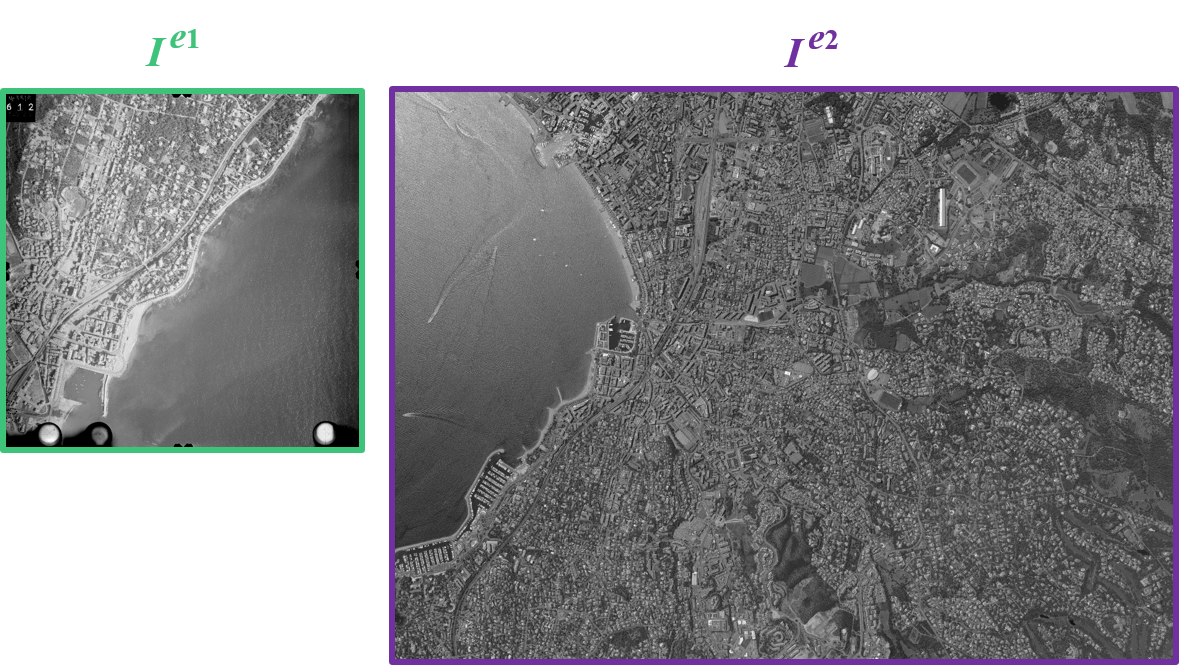
\includegraphics[width=1\columnwidth]{images/Chapitre4/example.png}
			\end{minipage}%
		}
		\subfigure[Demonstration of tile pairs]{
			\begin{minipage}[t]{1\linewidth}
				\centering
				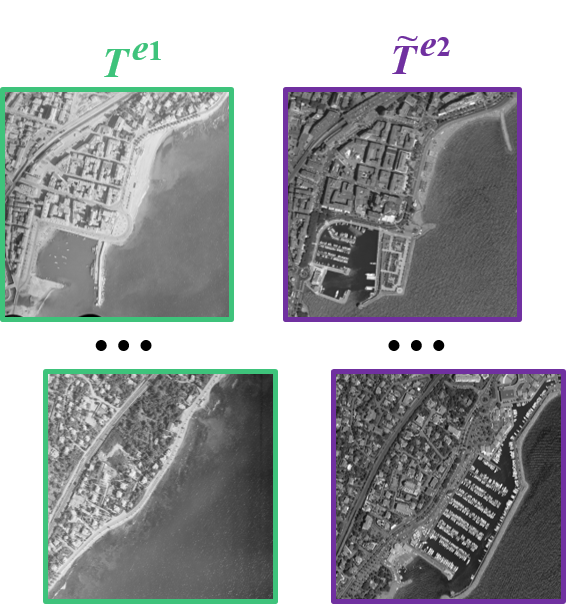
\includegraphics[width=1\columnwidth,trim=10 0 0 0,clip]{images/Chapitre4/patchexample.png}
			\end{minipage}%
		}
		%			\subfigure[Example of keypoint prediction]{
		%		\begin{minipage}[t]{1\linewidth}
		%			\centering
		%			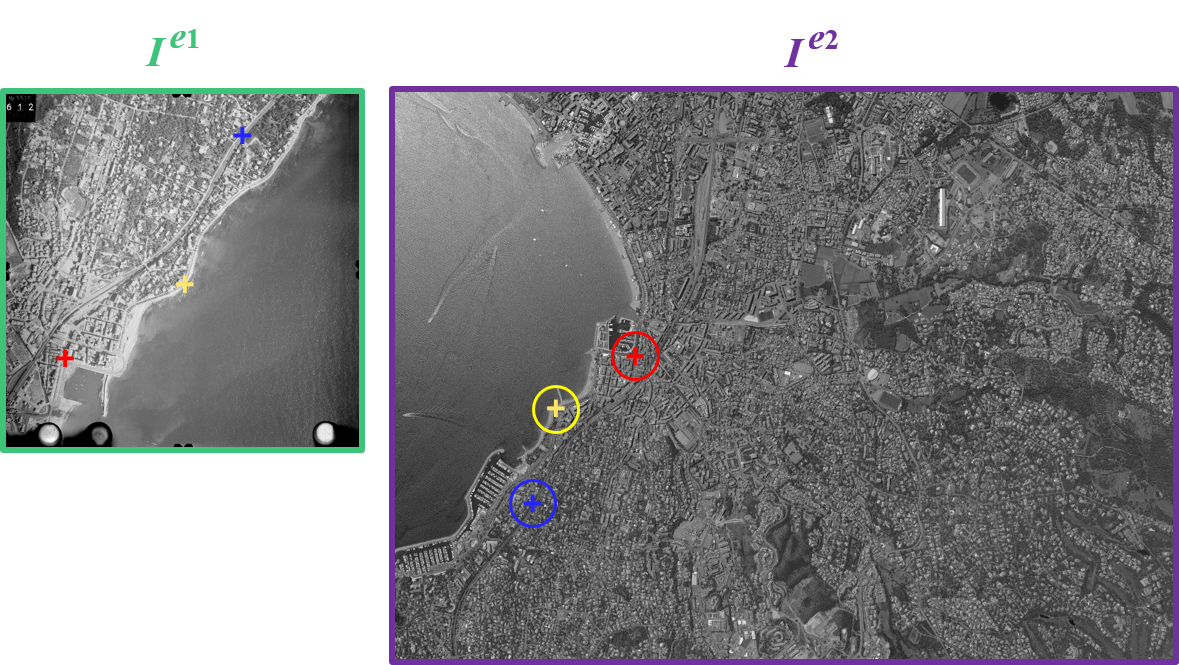
\includegraphics[width=1\columnwidth]{images/Chapitre4/guidedexample.png}
		%		\end{minipage}%
		%	}
		\caption{(a) Example demonstration of an image pair. The master image ($I^{e_1}$) and secondary image ($I^{e_2}$) are taken at Fr{\'e}jus in 1954 and 2014 individually. (b) Tile pairs resulted from \textit{one-to-one tiling scheme}, the tile zones before and after buffering are marked as green and blue rectangles.}
		\label{patchexample}
	\end{center}
\end{figure*}

\begin{figure*}[htbp]
	\begin{center}
		%\subfigure[Example of keypoint prediction]{
		%	\begin{minipage}[t]{1\linewidth}
				\centering
				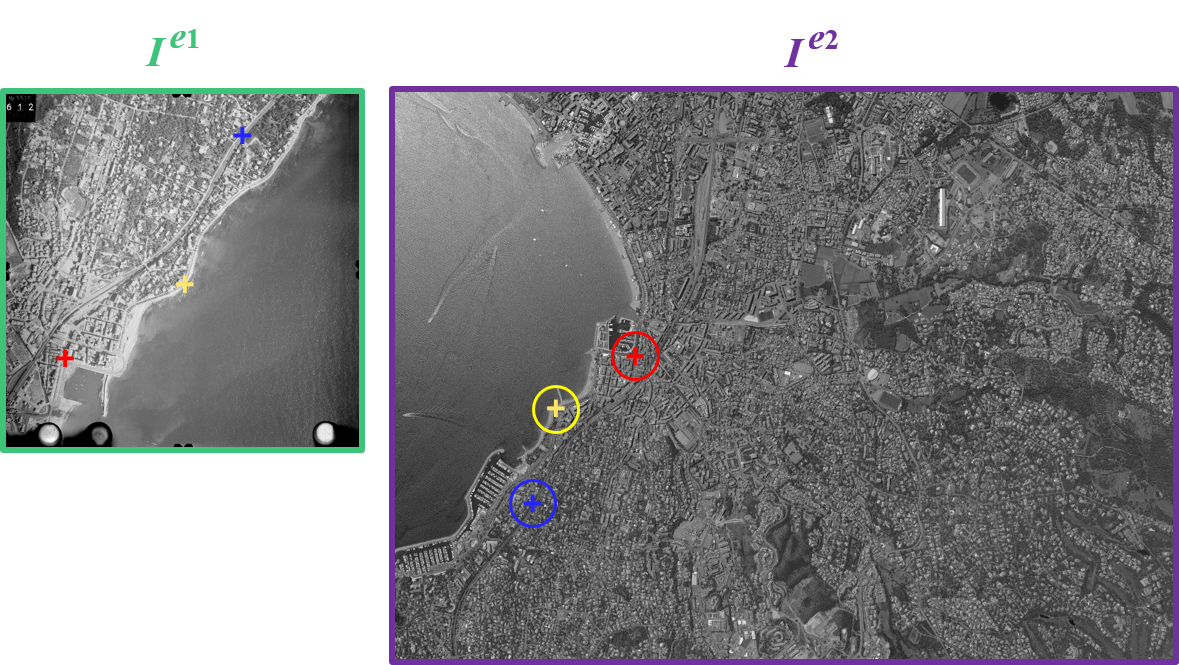
\includegraphics[width=1\columnwidth]{images/Chapitre4/guidedexample.png}
		%	\end{minipage}%
		%}
		\caption{Example demonstration of keypoint prediction (cross symbols) accompanied with search space (circles) on an image pair, the master image ($I^{e_1}$) and secondary image ($I^{e_2}$) are taken at Fr{\'e}jus in 1954 and 2014 individually.}
		\label{guidedexample}
	\end{center}
\end{figure*}

\subsubsection{Guided matching for hand-crafted features} 
The patch matching substitute orientated towards hand-crafted features is the guided matching, as shown in Figure~\ref{WorkflowPatch}(d). It leverages the positions of predicted keypoints, {the known scale ratio and rotation differences to narrow down the list of the matching candidates}. In our experiments, we use the SIFT points, but the pipeline is suitable to any hand-crafted extractor.
The strategy {is as follows}:\\
\begin{enumerate}
	\item {Compute the scale ratio $R_{scl}$ and the rotation $D_{rot}$ between two images by sequentially projecting the $I^{e_1}$ image corners to the co-registered DSM $D_{co}^{e_1}$ and to image $I^{e_2}$;} %\textcolor{red}{Project the image corners of $I^{e_1}$ to the co-registered DSM $D_{co}^{e_1}$, and back-project them to $I^{e_2}$ to estimate the scale ratio $R_{scl}$ and angle difference $D_{ang}$ between images $I^{e_1}$ and $I^{e_2}$.}
	\item Extract keypoints $\mathbf{K}^{e_1}$ in image $I^{e_1}$ and $\mathbf{K}^{e_2}$ in image $I^{e_2}$;
	\item Intersect the keypoints $\mathbf{K}^{e_1}$ with the co-registered DSM $D_{co}^{e_1}$;
	\item Back-project them to image $I^{e_2}$, giving rise to predicted keypoints $\widetilde{\mathbf{K}}^{e_2}$;
	\item Search for a subset of points in $\mathbf{K}^{e_2}$ located within a radius $S$ (100 pixels in our experiments) centered at the predicted positions $\widetilde{\mathbf{K}}^{e_2}$;%\textcolor{green}{(I don't use a distance threshold.)}
	\item {Remove candidate matches whose scales and rotations computed by SIFT are incoherent with $R_{scl}$ and $D_{rot}$ computed from image orientations and the co-registered DSM (i.e., step 1);}
	\item {Find the best match with mutual nearest neighbor and apply the first to second nearest neighbor ratio test~\cite{lowe2004distinctive}.}
\end{enumerate}
For better understanding, in Figure~\ref{guidedexample} we displayed an example of an inter-epoch image pair, with demonstration of keypoint prediction (cross symbols) accompanied with search space (circles) superposed on them.\\

\subsection{Get enhanced matches}
To compute enhanced matches, we apply a 3D-RANSAC filter on the previously obtained tentative matches. {More precisely, we do the following}: (1) for each match $M({\mathbf{K}^{e_1},\mathbf{K}^{e_2}})$, the keypoints $\mathbf{K}^{e_1}$ and $\mathbf{K}^{e_2}$ are projected onto DSM $D_{co}^{e_1}$ and $D_{ini}^{e_2}$ individually to get 3D points $M({\mathbf{G}^{e_1},\mathbf{G}^{e_2}})$; and (2) {the matches} $M({\mathbf{G}^{e_1},\mathbf{G}^{e_2}})$ are iteratively sampled to compute the 3D Helmert transformation RANSAC model:
\begin{equation}
\left [ \begin{array}{c}
{KG}_x^{e_2}\\
{KG}_y^{e_2}\\
{KG}_z^{e_2}
\end{array}
\right ] =\lambda \cdot \mathbf{R} \cdot {\left [ \begin{array}{c}
	{KG}_x^{e_1}\\
	{KG}_y^{e_1}\\
	{KG}_z^{e_1}
	\end{array}
	\right ]} + \left [ \begin{array}{c}
\Delta_x\\
\Delta_y\\
\Delta_z
\end{array}
\right ]. \label{eq:2DSim}
\end{equation}
where $\lambda$ is the scale factor, $\mathbf{R}$ is the rotation matrix and $\left [ \begin{array}{c}
\Delta_x, \Delta_y, \Delta_z
\end{array}
\right ]$ $^{^T}$ is the translation vector.
We set the number of RANSAC iterations to 1000, and consider matches within $T_r$ of its predicted position as inliers. In our experiment, {$T_r$ was set to 10$\times$$GSD$ where $GSD$ is the mean ground sampling distance in the coordinate frame of epoch ${e_2}$. This distance is computed as the ground distance between two adjacent image pixels.}

\subsection{Get final matches}
In the preceding step we got rid of a substantial number of outliers, however, we believe that not all outliers could be identified. Therefore we apply cross-correlation for final validation. Matches with their correlation scores below a predefined threshold (0.6 in our experiments) are discarded. The correlation window size was set to be large enough to take into account the context around a point (32$\times$32 pixels in our experiment). Figure~\ref{crossc} shows an example of a false match (red) eliminated by cross correlation, while the true match (blue) is kept.
\begin{figure*}[htbp]
	\begin{center}
		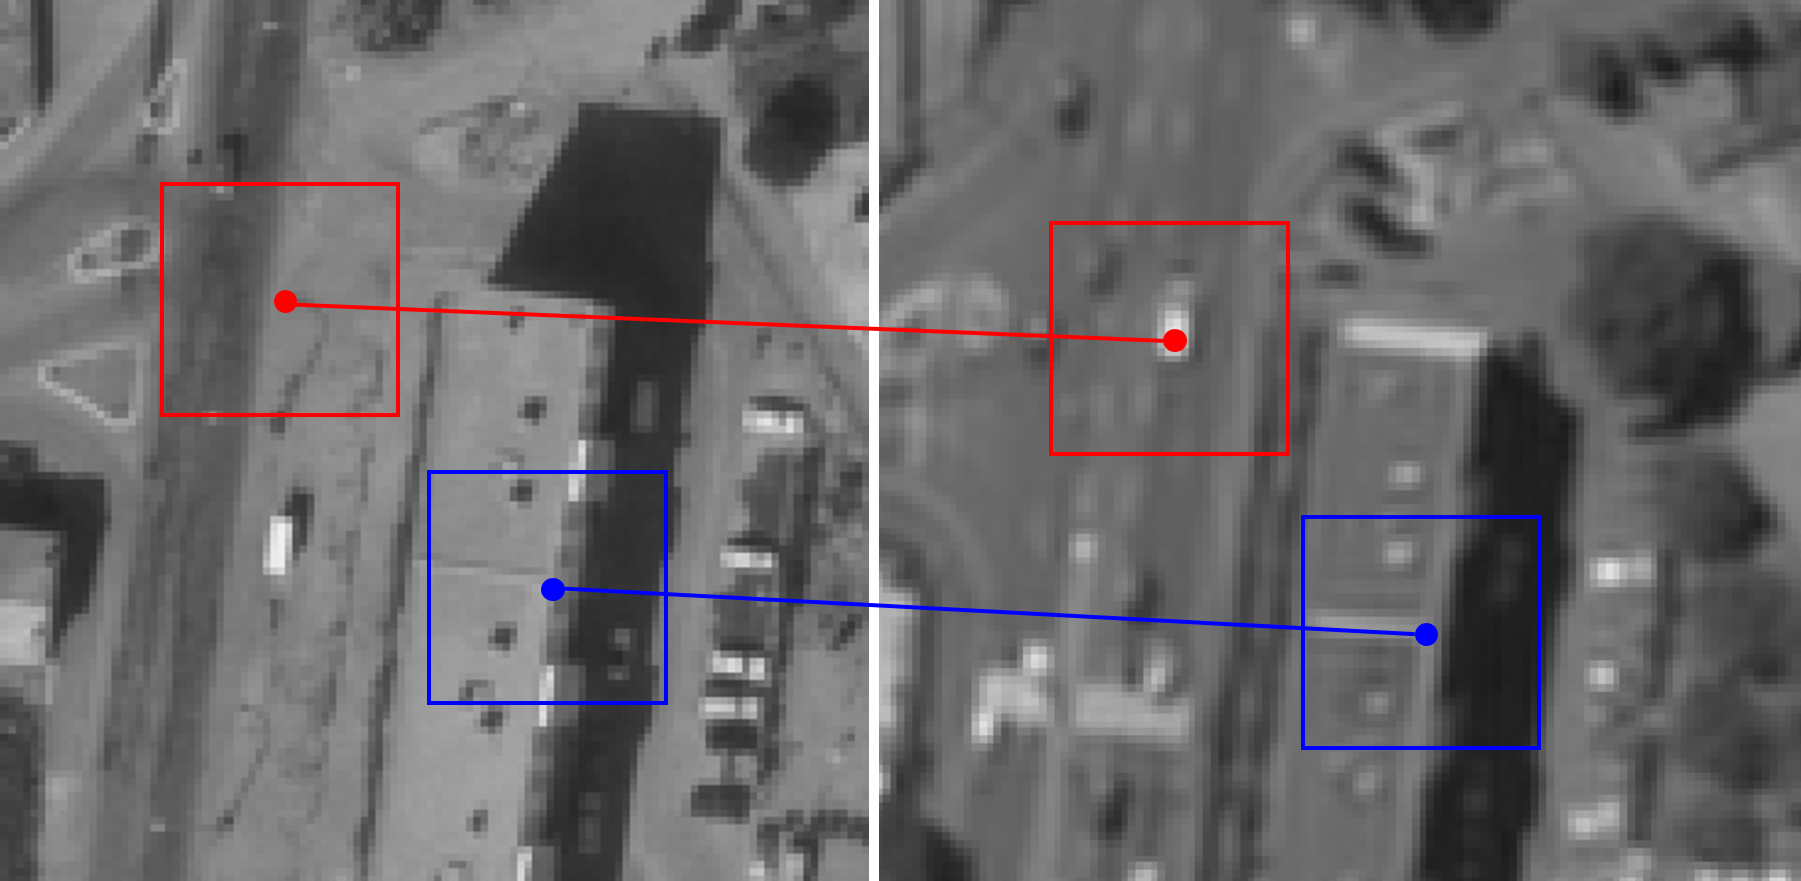
\includegraphics[width=0.8\columnwidth]{images/Chapitre4/tiept.png}
		\caption{Demonstration of the validation with cross-correlation. Considering poor quality of historical images, the window size (blue and red rectangles) was set to 32$\times$32 pixels. False match (red) is eliminated by cross correlation, while true match (blue) is kept.}
		\label{crossc}
	\end{center}
\end{figure*}

\subsection{Refine orientations}
Based on the intra-epoch and inter-epoch matches, a free network \ac{BBA} is performed to refine all the image orientations and camera calibrations. If the results need to be analyzed in a metric scale, a spatial similarity transformation will be performed to move the refined acquisitions in an arbitrary reference frame to a metric one. If the precise orientations for one of the epochs were known, their parameters will be fixed during the \ac{BBA} and the subsequent spatial similarity transformation will be skipped.
We adopted the Fraser model ~\cite{fraser1997digital} to calibrate the cameras and allowed image-dependent affine parameters, the remaining parameters were shared among all images.


\section{Experiments}
As described in the previous section, our precise matching pipeline consists of 3 main steps to get the tentative, enhanced and final matches. There are 2 alternatives for obtaining tentative matches (i.e. patch or guided matching), leading to 2 precise matching methods:\\
\begin{enumerate}
	\item \textit{Patch}: recover tentative matches with patch matching, followed by 3D RANSAC and cross correlation to remove outliers;
	\item \textit{Guided}: same as \textit{Patch}, except replacing patch matching with guided matching.
\end{enumerate}
For each dataset, we choose the rough co-registration results calculated with $SIFT_{DSM}$ and $SuperGlue_{DSM}$ individually (as they are the most robust methods for rough co-registration) to guide the precise matching \textit{Patch} or \textit{Guided}, leading to 4 sets of result, which are referred to as:\\
\begin{enumerate}
	\item $Patch_{SpGDSM}$
	\item $Guided_{SpGDSM}$
	\item $Patch_{SIFTDSM}$
	\item $Guided_{SIFTDSM}$
\end{enumerate}

\subsection{Implementation details}
Same as Section ~\ref{Implementationdetails}, all input images are downsampled by a factor of 3 beforehand to improve efficiency. To calculate the DSMs, we further downsample the images by a factor of 4 (different from 8 in Section ~\ref{Implementationdetails}), which amounts to a total downsampling factor of 12 with respect to the input images. For example, the images in Fr{\'e}jus 1970 are downsampled from [8766, 8763] to [730, 730] for calculating DSMs. 
Note that the DSMs serve 2 purposes in precise matching: (1) narrowing down the search space in precise matching, (2) providing 3D coordinates for 3D-RANSAC filter. A low resolution surface is good enough for these tasks and improves the efficiency.\\
To balance the number of the intra- and inter-epoch matches, we perform intra-epoch matches reduction available in MicMac~\cite{marc2016micmac}, followed by setting the relative observation weight in the \ac{BBA}, if necessary. The matches reduction algorithm maximizes good spatial distribution, points' multiplicity and low reprojection error, it also helps to speed up the \ac{BBA}.\\
Inter-epoch matches are extracted {for every possible combination of 2 epochs and finally merged}.\\


\subsection{Datasets}
We tested our precise matching methods on three sets of datasets: Fr{\'e}jus, Pezenas and Kobe. Details of the datasets are demonstrated in Section~\ref{Datasets}.\\
For Fr{\'e}jus and Kobe, we keep all the epochs for experiments, as the former displayed drastic scene changes and the latter witnessed an earthquake. For Pezenas, we choose aerial epoch 1971 and satellite epoch 2014 to test our precise matching and ignore other epochs to simplify the processing, since Pezenas is less challenging case.\\
The orientations of \ac{GT} epochs (i.e. Pezenas 2014 and Fr{\'e}jus 2014) were treated as fixed during the combined \ac{BBA} since they were accurately known \textit{a-priori}, while all the remaining orientations were considered as free parameters. At first, {interior orientation parameters} were shared among all images. Once stable initial values were known, interior parameters were further refined with image-dependent affine parameters. The affine component of the camera calibration is expected to model, at least partially, the shear of the analog film.\\
\subsection{Evaluation}
%Bar chart of recovered match numbers, Match visulization after CC (4 methods, 3 bars each. Kobe and Pezenas: one kit; Frejus: 6 kits)? DoD and statistic info, ground displacment, check pts? 
In order to evaluate the results qualitatively and quantitatively, the following criterias would be applied:\\
\begin{enumerate}
	\item \textbf{Matches visualization}. The number of tentative, enhanced and final matches would be displayed together in bar charts; in the meantime, the final matches would be visualized and demonstrated.
	%    \item Ground check points: the co-registered orientations calculated by our methods would be used to triangulate the ground check points and the coordinate differences \textcolor{red}{(explain the diff means the mean diff of x, y and z)} will be displayed. The better the epochs co-register, the smaller the difference is.
	\item \textbf{\ac{DoD}}. For each method, the refined orientations would be used to calculate DSMs in order to generate \ac{DoD}. The visualization of \ac{DoD} as well as the statistical information would be displayed. Since the orientations are refined with precise matches, \ac{DoD}s with dome effect mitigated or even eliminated are expected.\\
	For Pezenas and Fr\'ejus datasets, DoDs are calculated between historical epochs and the available \ac{GT} epochs. For Kobe dataset there is no \ac{GT} so we calculate the \ac{DoD} between 1991 and 1995 instead.\\
	%ideally the DoD should only display the scene changes without dome effect. If the dome effect appears, it indicates the systematic errors caused by poorly estimated camera parameters.   
	\item \textbf{Ground displacement}. For the dataset that witnessed an earthquake (i.e. Kobe), we: (1) calculate the DSMs; (2) orthorectify the images; and (3) perform 2D correlation of the respective orthophotos ~\cite{rosu2015measurement} to see whether we can observe the slip of the tectonic plate.
\end{enumerate}


\subsection{Comparison}
\subsubsection{Matches visualization}


\begin{figure*}[htbp]
	\begin{center}
		\subfigure[Common zone]{
			\begin{minipage}[t]{0.48\linewidth}
				\centering
				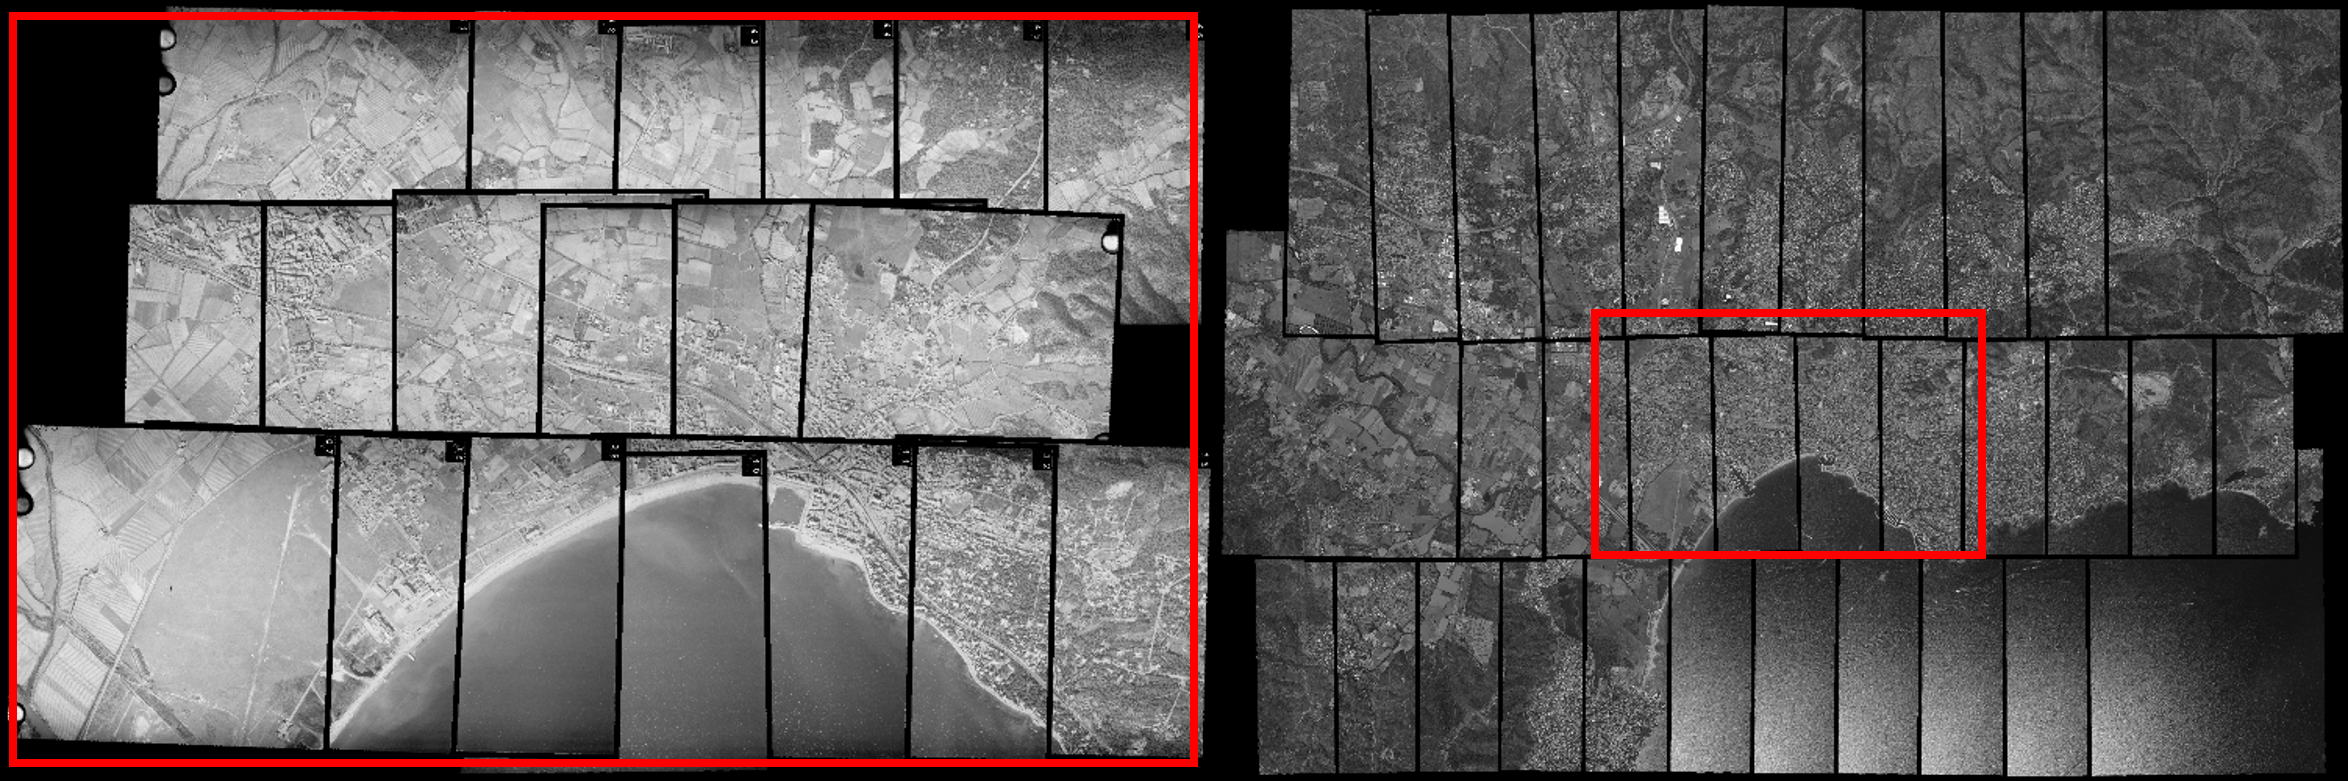
\includegraphics[width=6.8cm]{images/Chapitre3/Pseudo-Ortho-MEC-Malt_Tapas_1954_Ortho-MEC-Malt_2014.png}
			\end{minipage}%
		}
		\subfigure[Number of recovered matches]{
			\begin{minipage}[t]{0.48\linewidth}
				\centering
				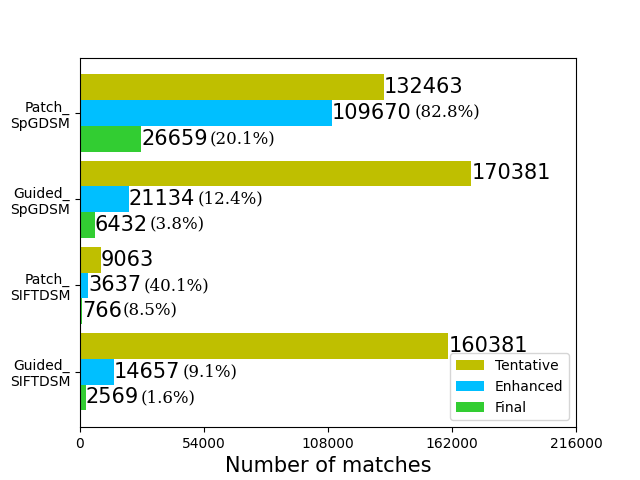
\includegraphics[width=5.8cm]{images/Chapitre4/PlotBarH-Frejus1954-2014.png}
			\end{minipage}%
		}
		\subfigure[$Patch_{SpGDSM}$]{
			\begin{minipage}[t]{0.48\linewidth}
				\centering
				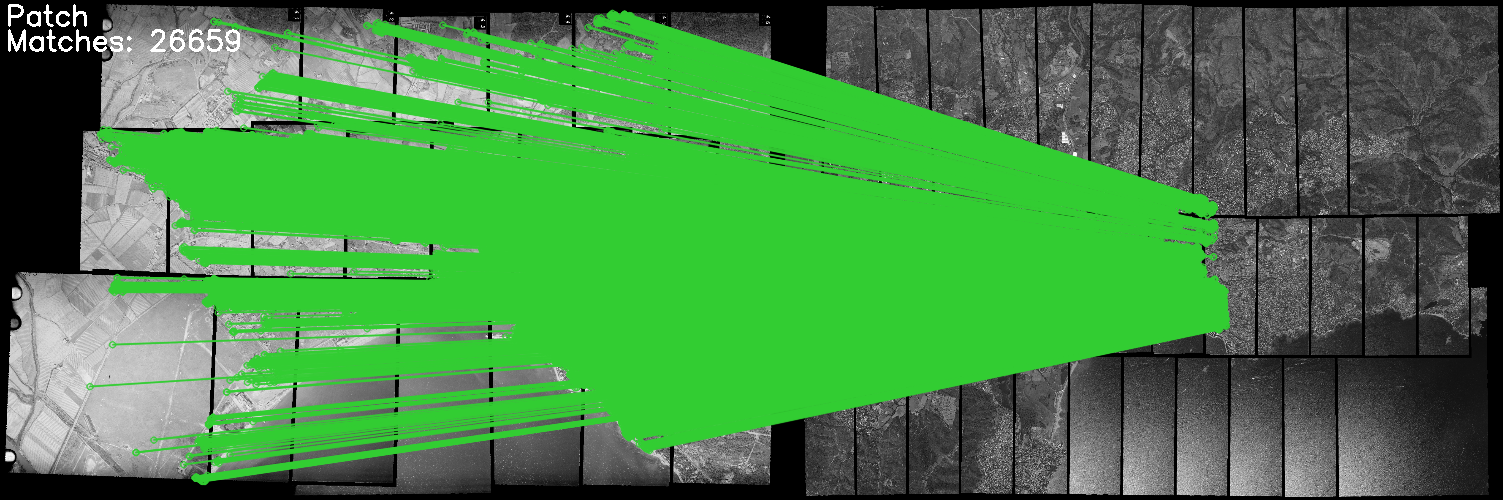
\includegraphics[width=6.8cm]{images/Chapitre4/Precise-SpGDSMHomol-1954-2014-SuperGlue-3DRANSAC-CrossCorrelation-PileImg_Ortho-MEC-Malt_Tapas_1954_Ortho-MEC-Malt_2014.png}
			\end{minipage}%
		}
		\subfigure[$Guided_{SpGDSM}$]{
			\begin{minipage}[t]{0.48\linewidth}
				\centering
				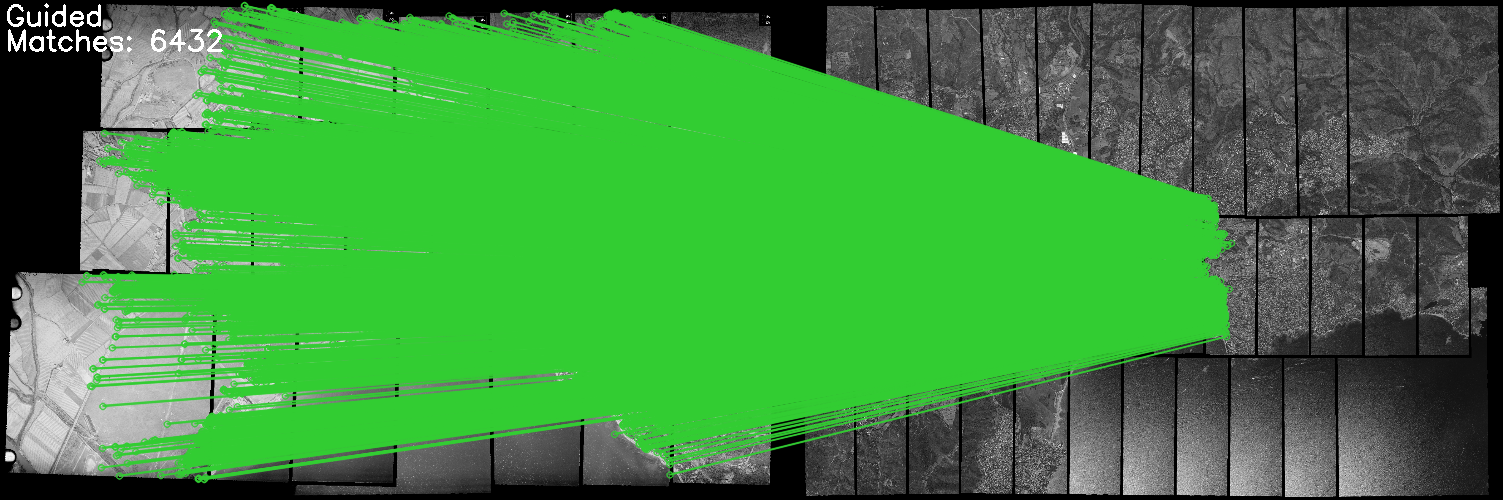
\includegraphics[width=6.8cm]{images/Chapitre4/Precise-SpGDSMHomol-1954-2014-GuidedSIFT-3DRANSAC-CrossCorrelation-PileImg_Ortho-MEC-Malt_Tapas_1954_Ortho-MEC-Malt_2014.png}
			\end{minipage}%
		}
		\subfigure[$Patch_{SIFTDSM}$]{
			\begin{minipage}[t]{0.48\linewidth}
				\centering
				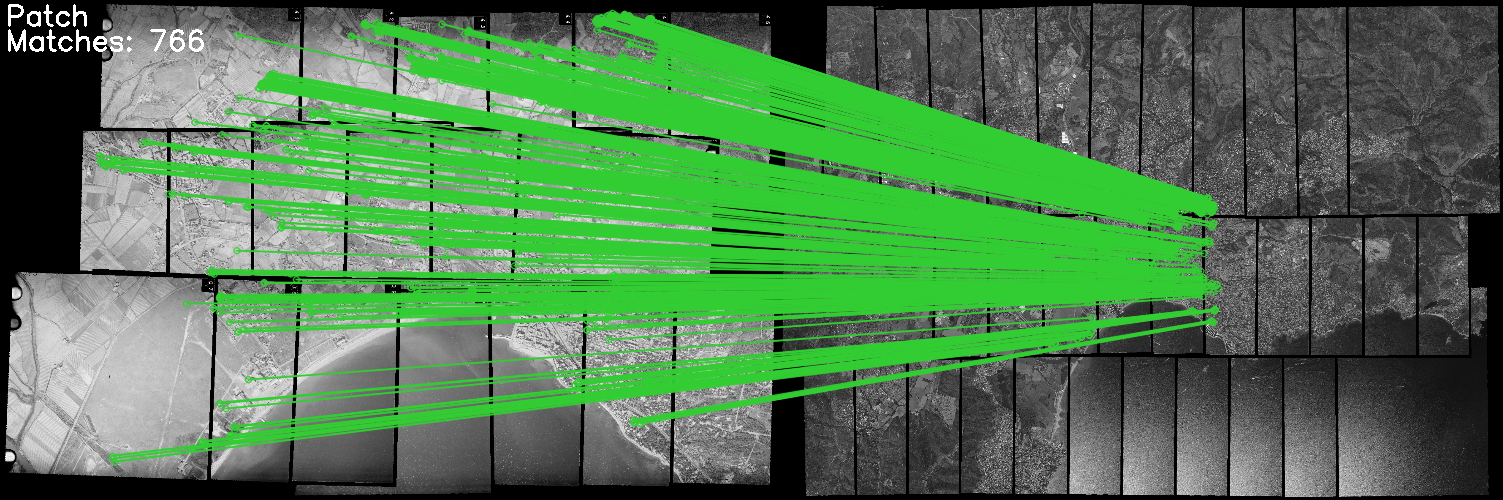
\includegraphics[width=6.8cm]{images/Chapitre4/Precise-SIFTDSMHomol-1954-2014-SuperGlue-3DRANSAC-CrossCorrelation-PileImg_Ortho-MEC-Malt_Tapas_1954_Ortho-MEC-Malt_2014.png}
			\end{minipage}%
		}
		\subfigure[$Guided_{SIFTDSM}$]{
			\begin{minipage}[t]{0.48\linewidth}
				\centering
				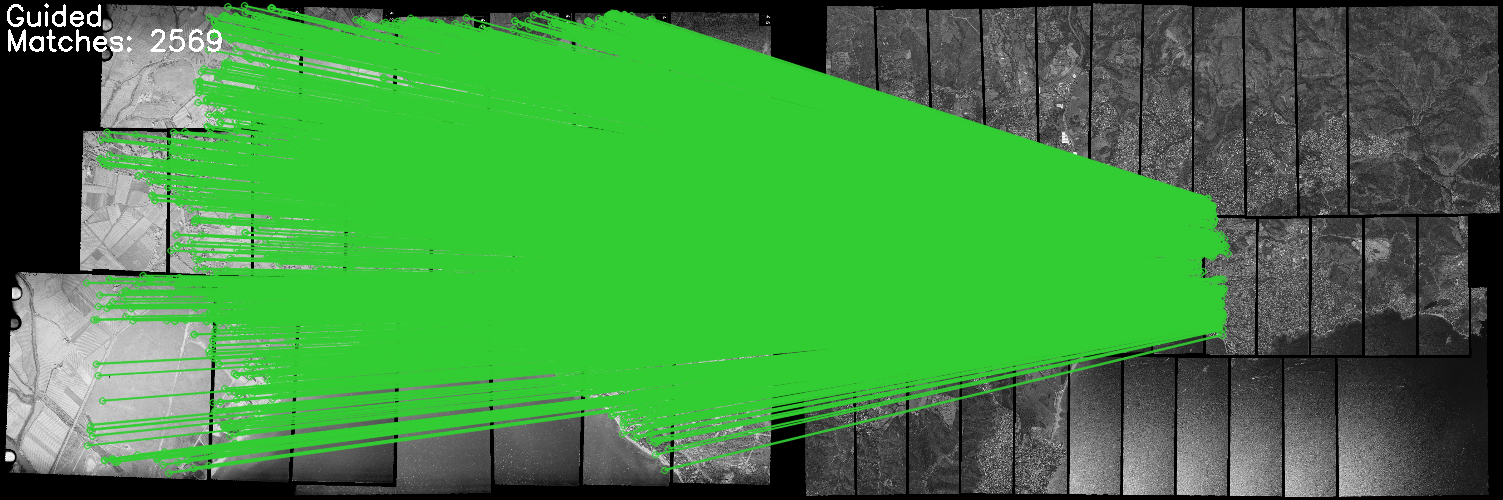
\includegraphics[width=6.8cm]{images/Chapitre4/Precise-SIFTDSMHomol-1954-2014-GuidedSIFT-3DRANSAC-CrossCorrelation-PileImg_Ortho-MEC-Malt_Tapas_1954_Ortho-MEC-Malt_2014.png}
			\end{minipage}%
		}
		\caption{Precise matching visualization of \textbf{Fr{\'e}jus 1954 and 2014}. (a) Image pairs to be matched, with red rectangles indicating the common zone. (b) Numbers of tentative, enhanced and final matches recovered with $Patch_{SpGDSM}$, $Guided_{SpGDSM}$, $Patch_{SIFTDSM}$ and $Guided_{SIFTDSM}$ individually. (c-f) Visualization of final matches recovered with $Patch_{SpGDSM}$, $Guided_{SpGDSM}$, $Patch_{SIFTDSM}$ and $Guided_{SIFTDSM}$ individually.}
		\label{MatchVizFrejus1954-2014}
	\end{center}
\end{figure*} 


\begin{figure*}[htbp]
	\begin{center}
		\subfigure[Common zone]{
			\begin{minipage}[t]{0.48\linewidth}
				\centering
				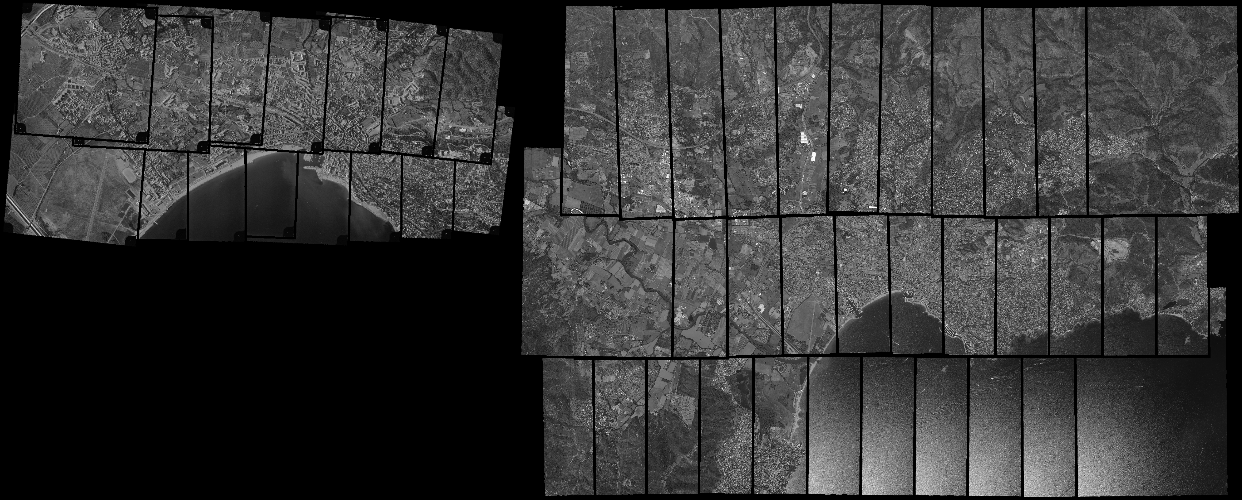
\includegraphics[width=6.8cm]{images/Chapitre3/Pseudo-Ortho-MEC-Malt_Tapas_1966_Ortho-MEC-Malt_2014.png}
			\end{minipage}%
		}
		\subfigure[Number of recovered matches]{
			\begin{minipage}[t]{0.48\linewidth}
				\centering
				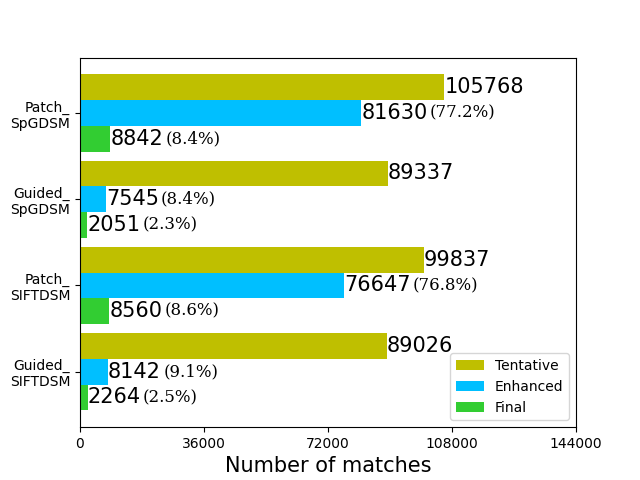
\includegraphics[width=5.8cm]{images/Chapitre4/PlotBarH-Frejus1966-2014.png}
			\end{minipage}%
		}
		\subfigure[$Patch_{SpGDSM}$]{
			\begin{minipage}[t]{0.48\linewidth}
				\centering
				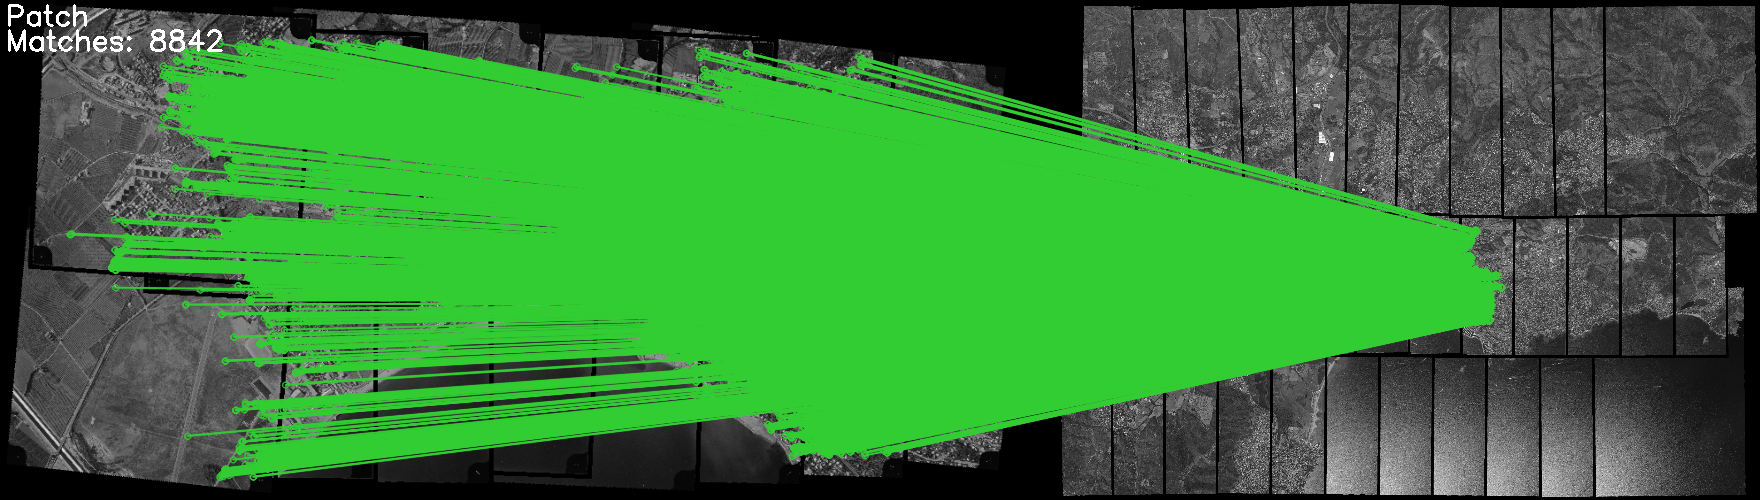
\includegraphics[width=6.8cm]{images/Chapitre4/Precise-SpGDSMHomol-1966-2014-SuperGlue-3DRANSAC-CrossCorrelation-PileImg_Ortho-MEC-Malt_Tapas_1966_Ortho-MEC-Malt_2014.png}
			\end{minipage}%
		}
		\subfigure[$Guided_{SpGDSM}$]{
			\begin{minipage}[t]{0.48\linewidth}
				\centering
				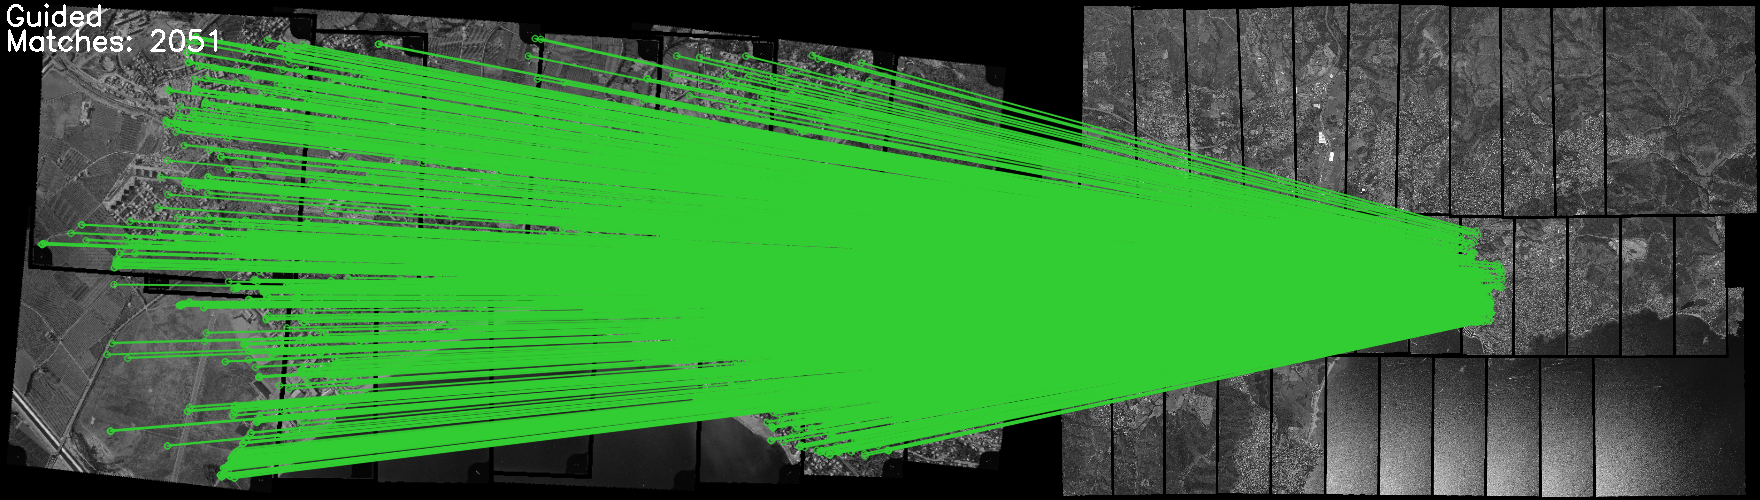
\includegraphics[width=6.8cm]{images/Chapitre4/Precise-SpGDSMHomol-1966-2014-GuidedSIFT-3DRANSAC-CrossCorrelation-PileImg_Ortho-MEC-Malt_Tapas_1966_Ortho-MEC-Malt_2014.png}
			\end{minipage}%
		}
		\subfigure[$Patch_{SIFTDSM}$]{
			\begin{minipage}[t]{0.48\linewidth}
				\centering
				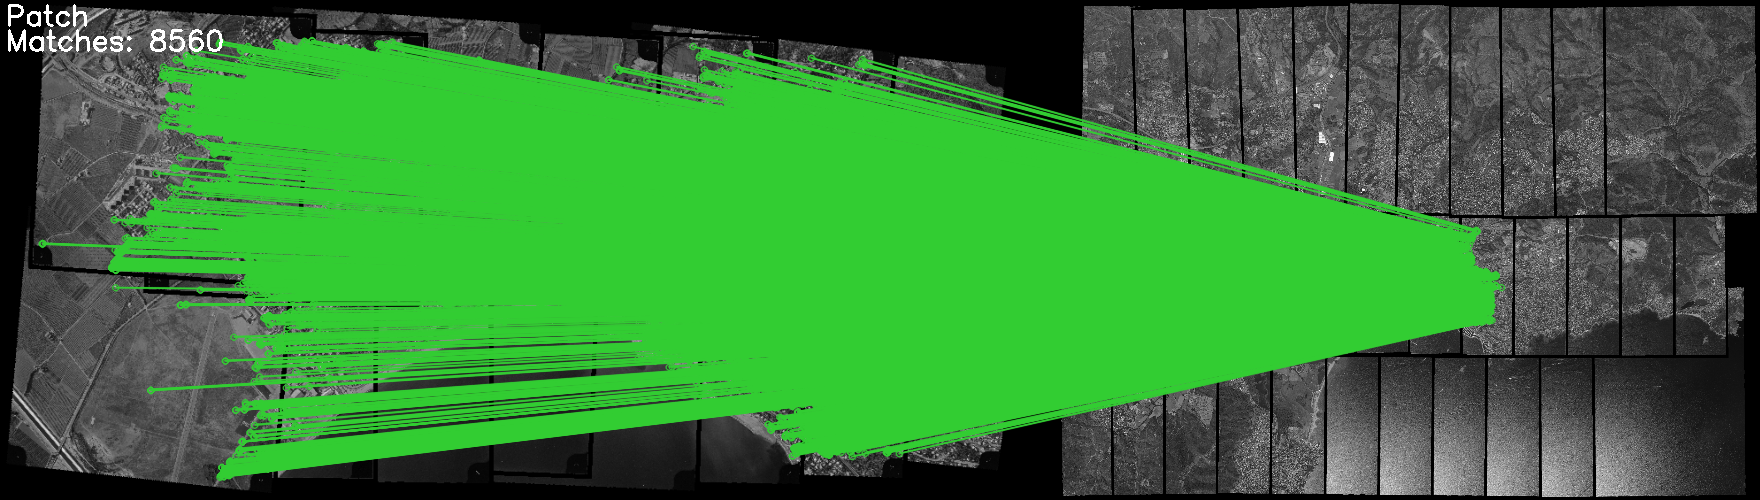
\includegraphics[width=6.8cm]{images/Chapitre4/Precise-SIFTDSMHomol-1966-2014-SuperGlue-3DRANSAC-CrossCorrelation-PileImg_Ortho-MEC-Malt_Tapas_1966_Ortho-MEC-Malt_2014.png}
			\end{minipage}%
		}
		\subfigure[$Guided_{SIFTDSM}$]{
			\begin{minipage}[t]{0.48\linewidth}
				\centering
				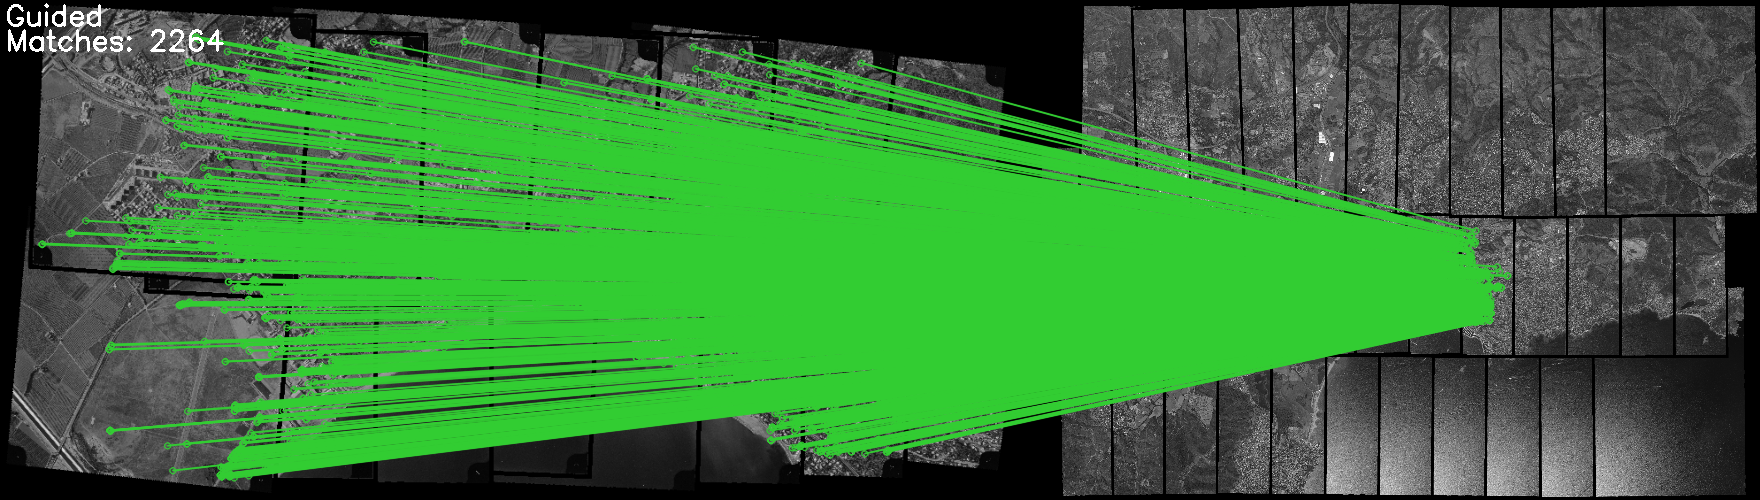
\includegraphics[width=6.8cm]{images/Chapitre4/Precise-SIFTDSMHomol-1966-2014-GuidedSIFT-3DRANSAC-CrossCorrelation-PileImg_Ortho-MEC-Malt_Tapas_1966_Ortho-MEC-Malt_2014.png}
			\end{minipage}%
		}
		\caption{Precise matching visualization of \textbf{Fr{\'e}jus 1966 and 2014}. (a) Image pairs to be matched, with red rectangles indicating the common zone. (b) Numbers of tentative, enhanced and final matches recovered with $Patch_{SpGDSM}$, $Guided_{SpGDSM}$, $Patch_{SIFTDSM}$ and $Guided_{SIFTDSM}$ individually. (c-f) Visualization of final matches recovered with $Patch_{SpGDSM}$, $Guided_{SpGDSM}$, $Patch_{SIFTDSM}$ and $Guided_{SIFTDSM}$ individually.}
		\label{MatchVizFrejus1966-2014}
	\end{center}
\end{figure*} 


\begin{figure*}[htbp]
	\begin{center}
		\subfigure[Common zone]{
			\begin{minipage}[t]{0.48\linewidth}
				\centering
				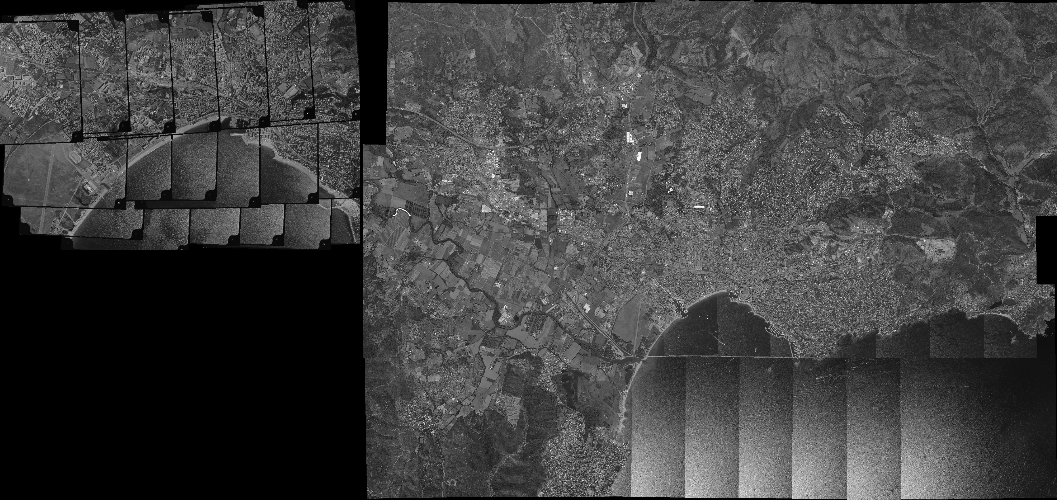
\includegraphics[width=6.8cm]{images/Chapitre3/Pseudo-Ortho-MEC-Malt_Tapas_1970_Ortho-MEC-Malt_2014.png}
			\end{minipage}%
		}
		\subfigure[Number of recovered matches]{
			\begin{minipage}[t]{0.48\linewidth}
				\centering
				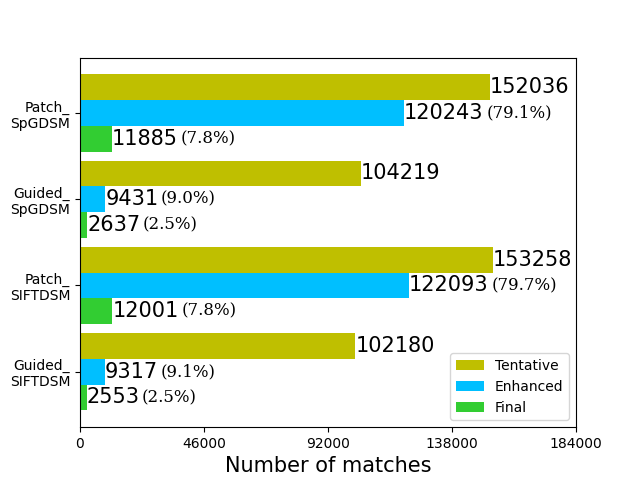
\includegraphics[width=5.8cm]{images/Chapitre4/PlotBarH-Frejus1970-2014.png}
			\end{minipage}%
		}
		\subfigure[$Patch_{SpGDSM}$]{
			\begin{minipage}[t]{0.48\linewidth}
				\centering
				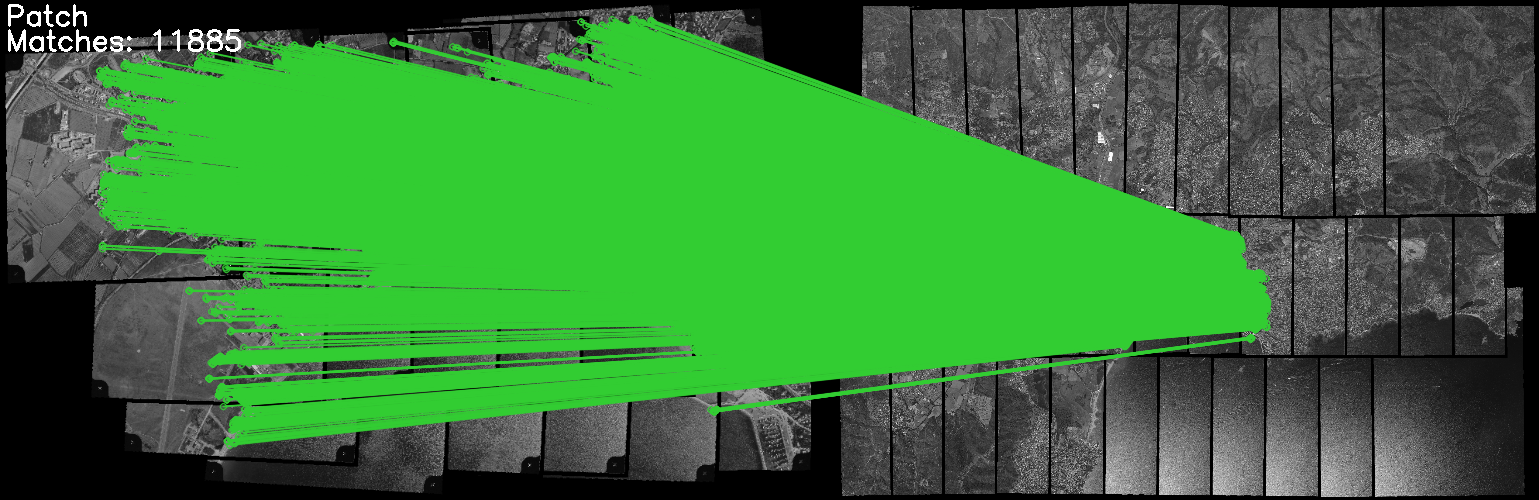
\includegraphics[width=6.8cm]{images/Chapitre4/Precise-SpGDSMHomol-1970-2014-SuperGlue-3DRANSAC-CrossCorrelation-PileImg_Ortho-MEC-Malt_Tapas_1970_Ortho-MEC-Malt_2014.png}
			\end{minipage}%
		}
		\subfigure[$Guided_{SpGDSM}$]{
			\begin{minipage}[t]{0.48\linewidth}
				\centering
				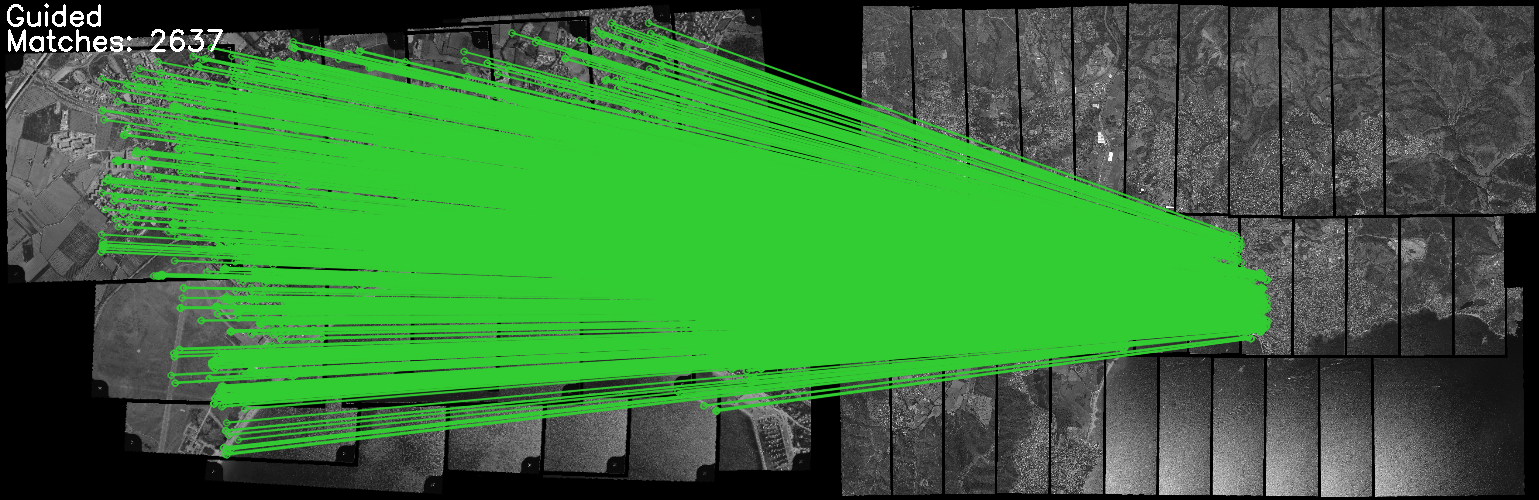
\includegraphics[width=6.8cm]{images/Chapitre4/Precise-SpGDSMHomol-1970-2014-GuidedSIFT-3DRANSAC-CrossCorrelation-PileImg_Ortho-MEC-Malt_Tapas_1970_Ortho-MEC-Malt_2014.png}
			\end{minipage}%
		}
		\subfigure[$Patch_{SIFTDSM}$]{
			\begin{minipage}[t]{0.48\linewidth}
				\centering
				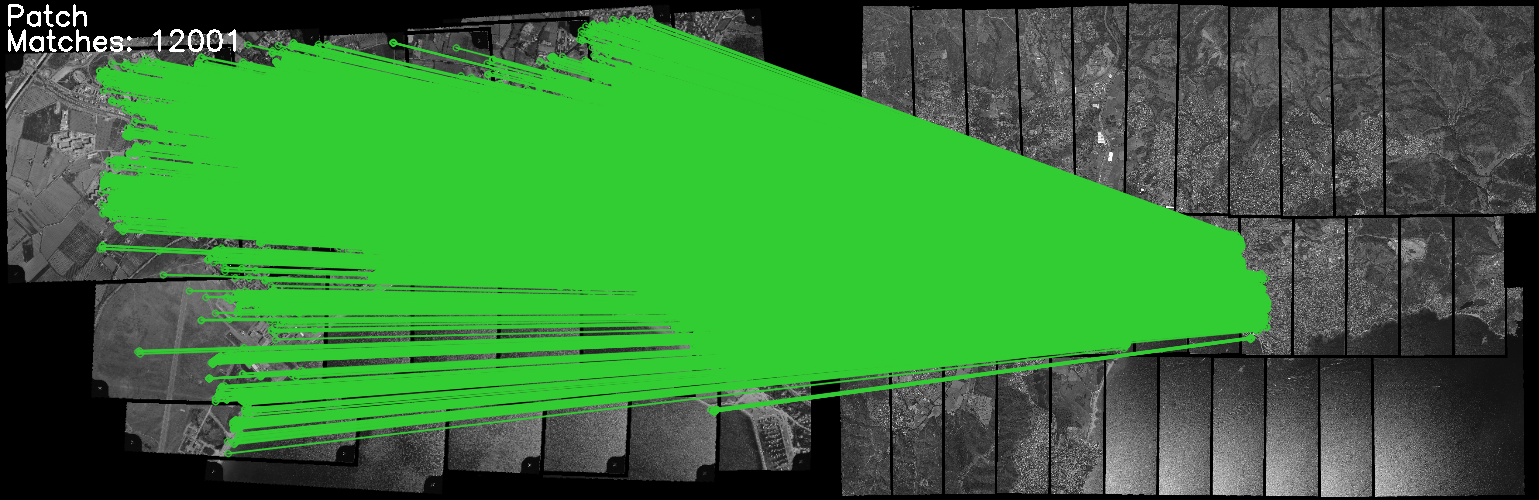
\includegraphics[width=6.8cm]{images/Chapitre4/Precise-SIFTDSMHomol-1970-2014-SuperGlue-3DRANSAC-CrossCorrelation-PileImg_Ortho-MEC-Malt_Tapas_1970_Ortho-MEC-Malt_2014.png}
			\end{minipage}%
		}
		\subfigure[$Guided_{SIFTDSM}$]{
			\begin{minipage}[t]{0.48\linewidth}
				\centering
				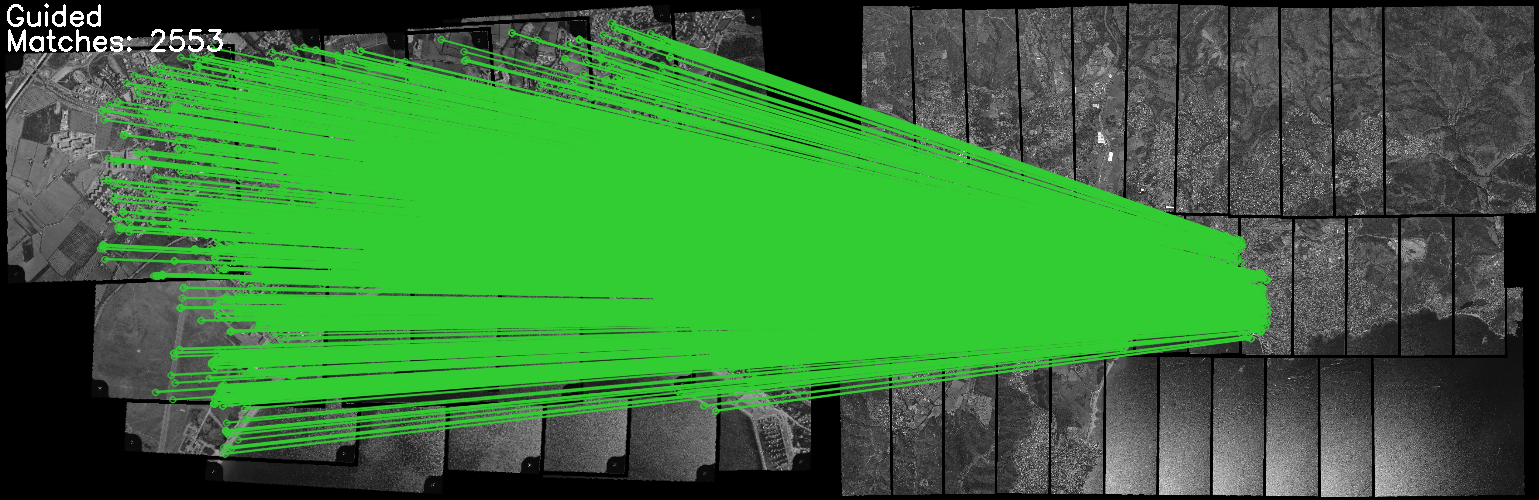
\includegraphics[width=6.8cm]{images/Chapitre4/Precise-SIFTDSMHomol-1970-2014-GuidedSIFT-3DRANSAC-CrossCorrelation-PileImg_Ortho-MEC-Malt_Tapas_1970_Ortho-MEC-Malt_2014.png}
			\end{minipage}%
		}
		\caption{Precise matching visualization of \textbf{Fr{\'e}jus 1970 and 2014}. (a) Image pairs to be matched, with red rectangles indicating the common zone. (b) Numbers of tentative, enhanced and final matches recovered with $Patch_{SpGDSM}$, $Guided_{SpGDSM}$, $Patch_{SIFTDSM}$ and $Guided_{SIFTDSM}$ individually. (c-f) Visualization of final matches recovered with $Patch_{SpGDSM}$, $Guided_{SpGDSM}$, $Patch_{SIFTDSM}$ and $Guided_{SIFTDSM}$ individually.}
		\label{MatchVizFrejus1970-2014}
	\end{center}
\end{figure*} 

%%%%%%%%%%%%%%%%%%Frejus histo

\begin{figure*}[htbp]
	\begin{center}
		\subfigure[Common zone]{
			\begin{minipage}[t]{0.48\linewidth}
				\centering
				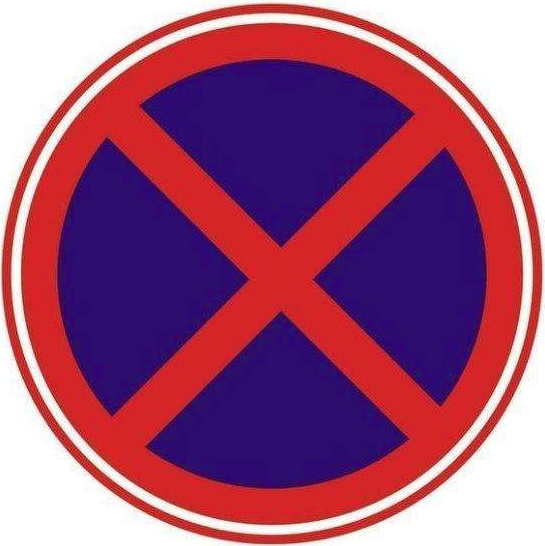
\includegraphics[width=6.8cm]{images/Chapitre4/Pseudo-Ortho-MEC-Malt_Tapas_1954_Ortho-MEC-Malt_Tapas_1970.png}
			\end{minipage}%
		}
		\subfigure[Number of recovered matches]{
			\begin{minipage}[t]{0.48\linewidth}
				\centering
				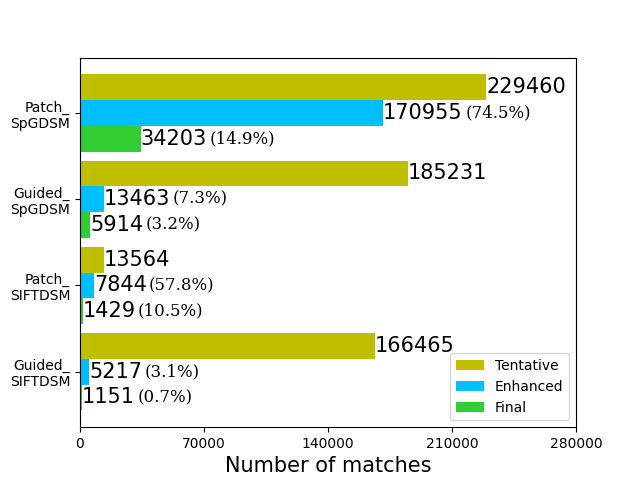
\includegraphics[width=5.8cm]{images/Chapitre4/PlotBarH-Frejus1954-1970.png}
			\end{minipage}%
		}
		\subfigure[$Patch_{SpGDSM}$]{
			\begin{minipage}[t]{0.48\linewidth}
				\centering
				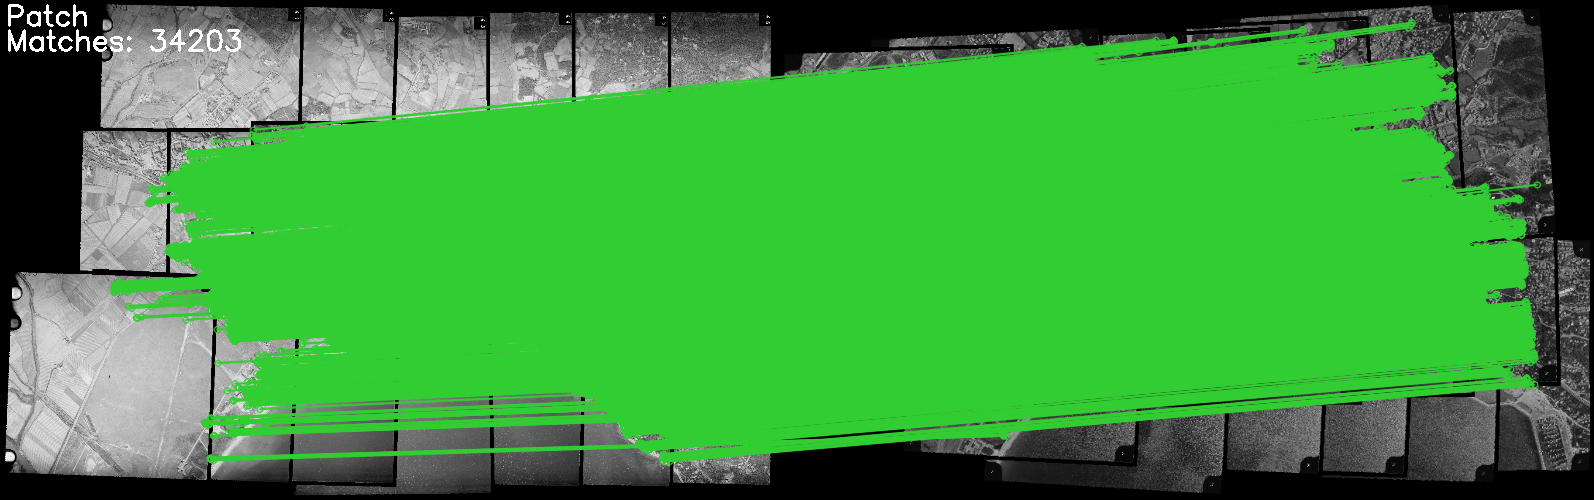
\includegraphics[width=6.8cm]{images/Chapitre4/Precise-SpGDSMHomol-1954-1970-SuperGlue-3DRANSAC-CrossCorrelation-PileImg_Ortho-MEC-Malt_Tapas_1954_Ortho-MEC-Malt_Tapas_1970.png}
			\end{minipage}%
		}
		\subfigure[$Guided_{SpGDSM}$]{
			\begin{minipage}[t]{0.48\linewidth}
				\centering
				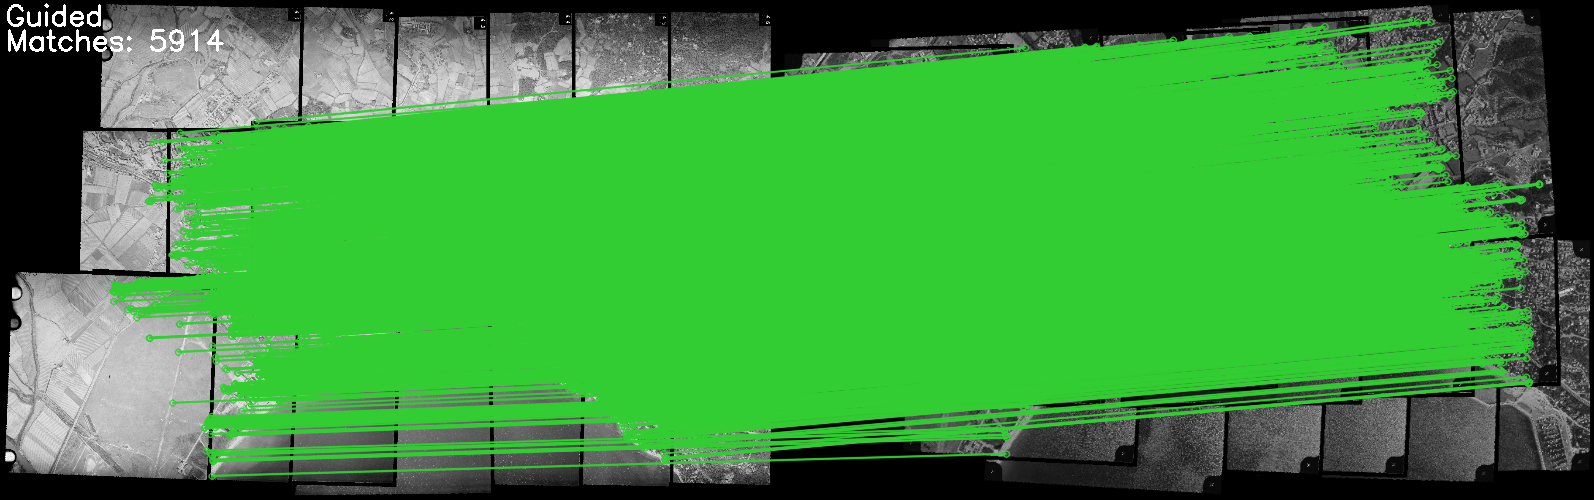
\includegraphics[width=6.8cm]{images/Chapitre4/Precise-SpGDSMHomol-1954-1970-GuidedSIFT-3DRANSAC-CrossCorrelation-PileImg_Ortho-MEC-Malt_Tapas_1954_Ortho-MEC-Malt_Tapas_1970.png}
			\end{minipage}%
		}
		\subfigure[$Patch_{SIFTDSM}$]{
			\begin{minipage}[t]{0.48\linewidth}
				\centering
				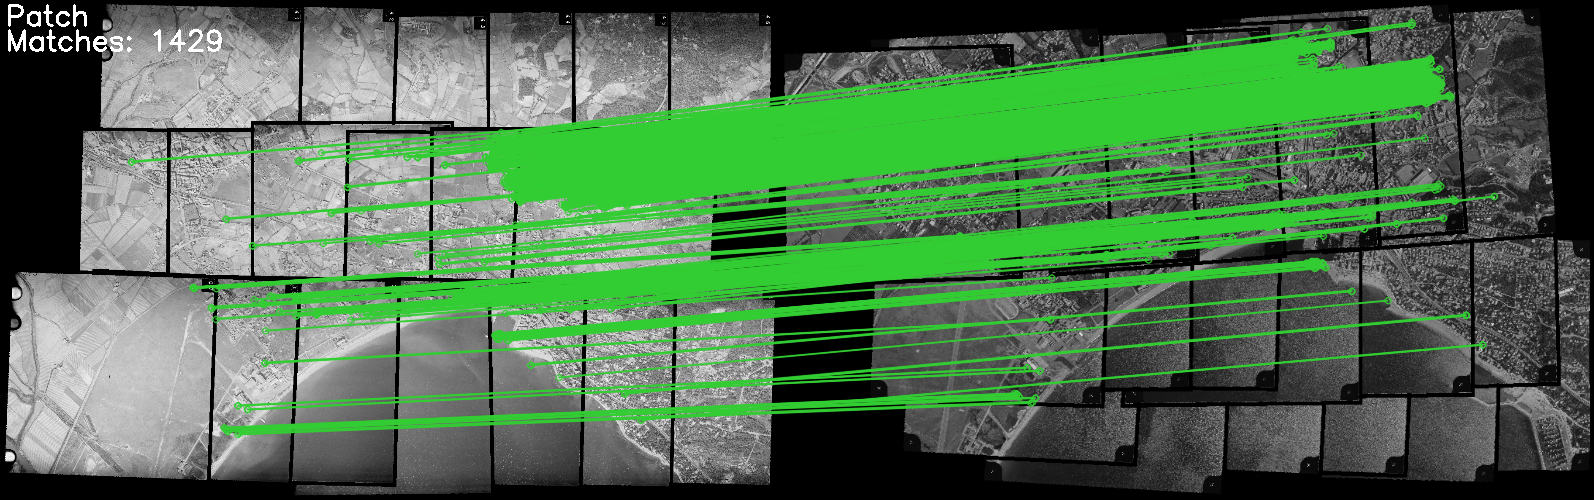
\includegraphics[width=6.8cm]{images/Chapitre4/Precise-SIFTDSMHomol-1954-1970-SuperGlue-3DRANSAC-CrossCorrelation-PileImg_Ortho-MEC-Malt_Tapas_1954_Ortho-MEC-Malt_Tapas_1970.png}
			\end{minipage}%
		}
		\subfigure[$Guided_{SIFTDSM}$]{
			\begin{minipage}[t]{0.48\linewidth}
				\centering
				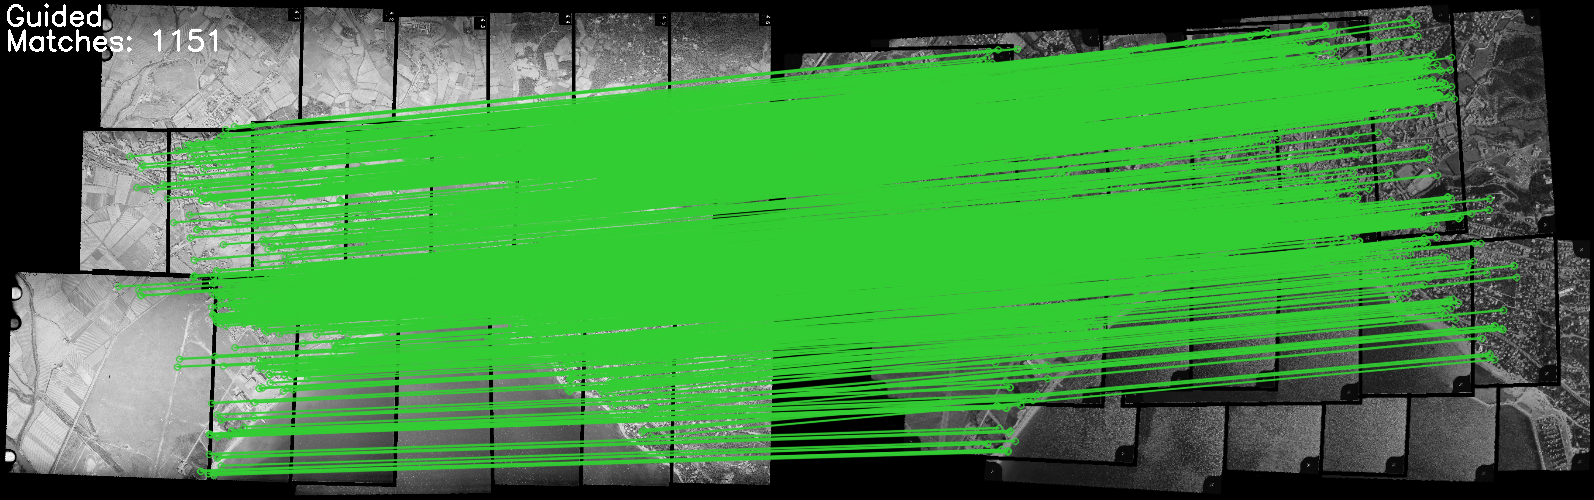
\includegraphics[width=6.8cm]{images/Chapitre4/Precise-SIFTDSMHomol-1954-1970-GuidedSIFT-3DRANSAC-CrossCorrelation-PileImg_Ortho-MEC-Malt_Tapas_1954_Ortho-MEC-Malt_Tapas_1970.png}
			\end{minipage}%
		}
		\caption{Precise matching visualization of \textbf{Fr{\'e}jus 1954 and 1970}. (a) Image pairs to be matched, with red rectangles indicating the common zone. (b) Numbers of tentative, enhanced and final matches recovered with $Patch_{SpGDSM}$, $Guided_{SpGDSM}$, $Patch_{SIFTDSM}$ and $Guided_{SIFTDSM}$ individually. (c-f) Visualization of final matches recovered with $Patch_{SpGDSM}$, $Guided_{SpGDSM}$, $Patch_{SIFTDSM}$ and $Guided_{SIFTDSM}$ individually.}
		\label{MatchVizFrejus1954-1970}
	\end{center}
\end{figure*} 



\begin{figure*}[htbp]
	\begin{center}
		\subfigure[Common zone]{
			\begin{minipage}[t]{0.48\linewidth}
				\centering
				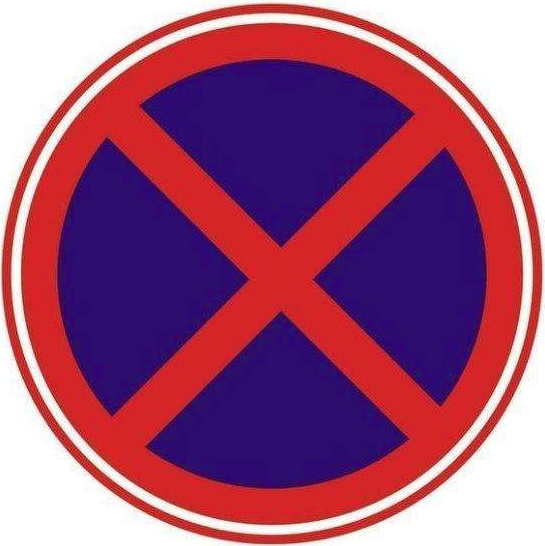
\includegraphics[width=6.8cm]{images/Chapitre4/Pseudo-Ortho-MEC-Malt_Tapas_1966_Ortho-MEC-Malt_Tapas_1970.png}
			\end{minipage}%
		}
		\subfigure[Number of recovered matches]{
			\begin{minipage}[t]{0.48\linewidth}
				\centering
				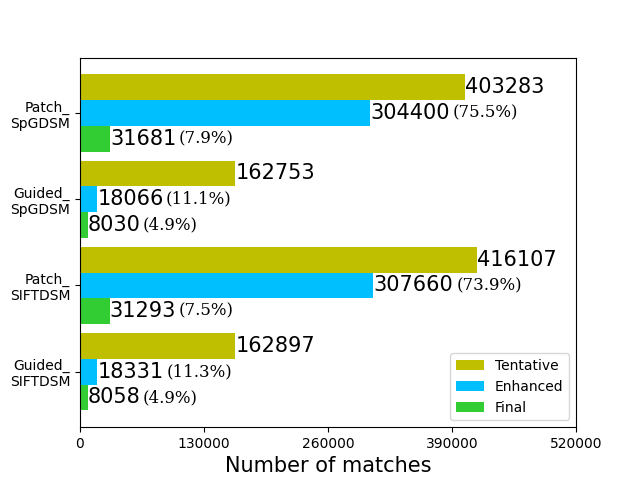
\includegraphics[width=5.8cm]{images/Chapitre4/PlotBarH-Frejus1966-1970.png}
			\end{minipage}%
		}
		\subfigure[$Patch_{SpGDSM}$]{
			\begin{minipage}[t]{0.48\linewidth}
				\centering
				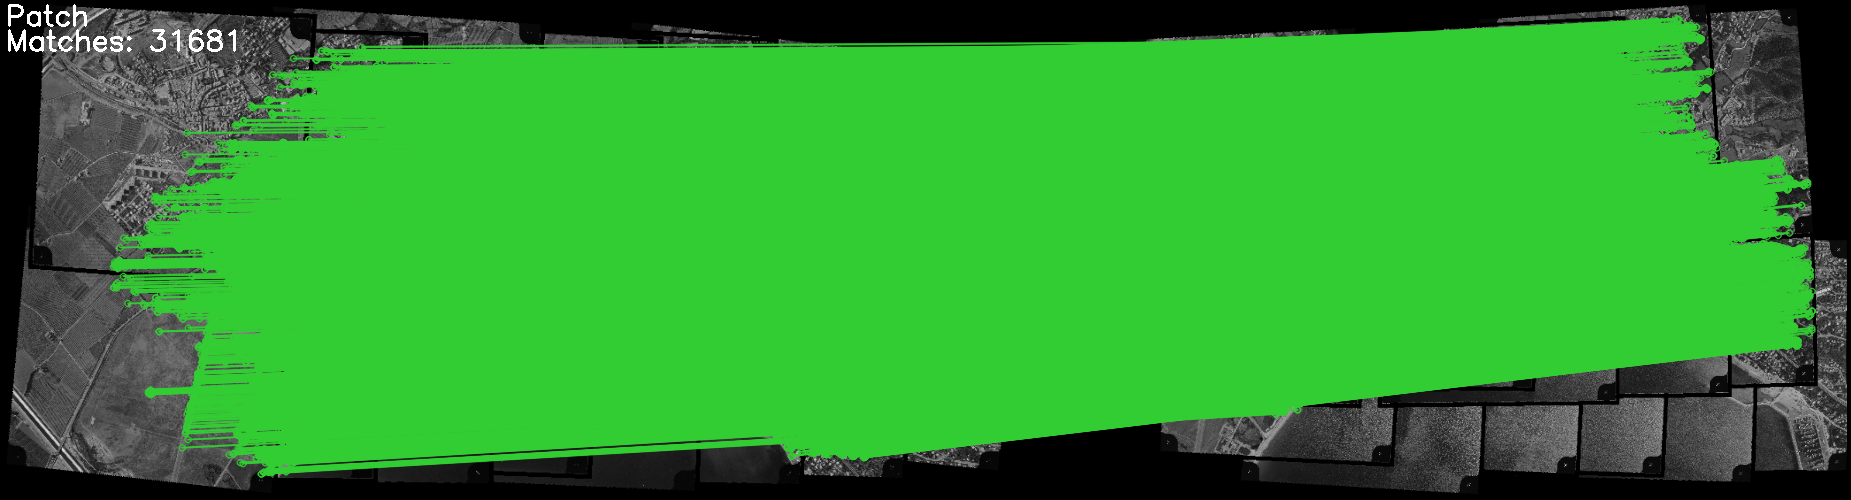
\includegraphics[width=6.8cm]{images/Chapitre4/Precise-SpGDSMHomol-1966-1970-SuperGlue-3DRANSAC-CrossCorrelation-PileImg_Ortho-MEC-Malt_Tapas_1966_Ortho-MEC-Malt_Tapas_1970.png}
			\end{minipage}%
		}
		\subfigure[$Guided_{SpGDSM}$]{
			\begin{minipage}[t]{0.48\linewidth}
				\centering
				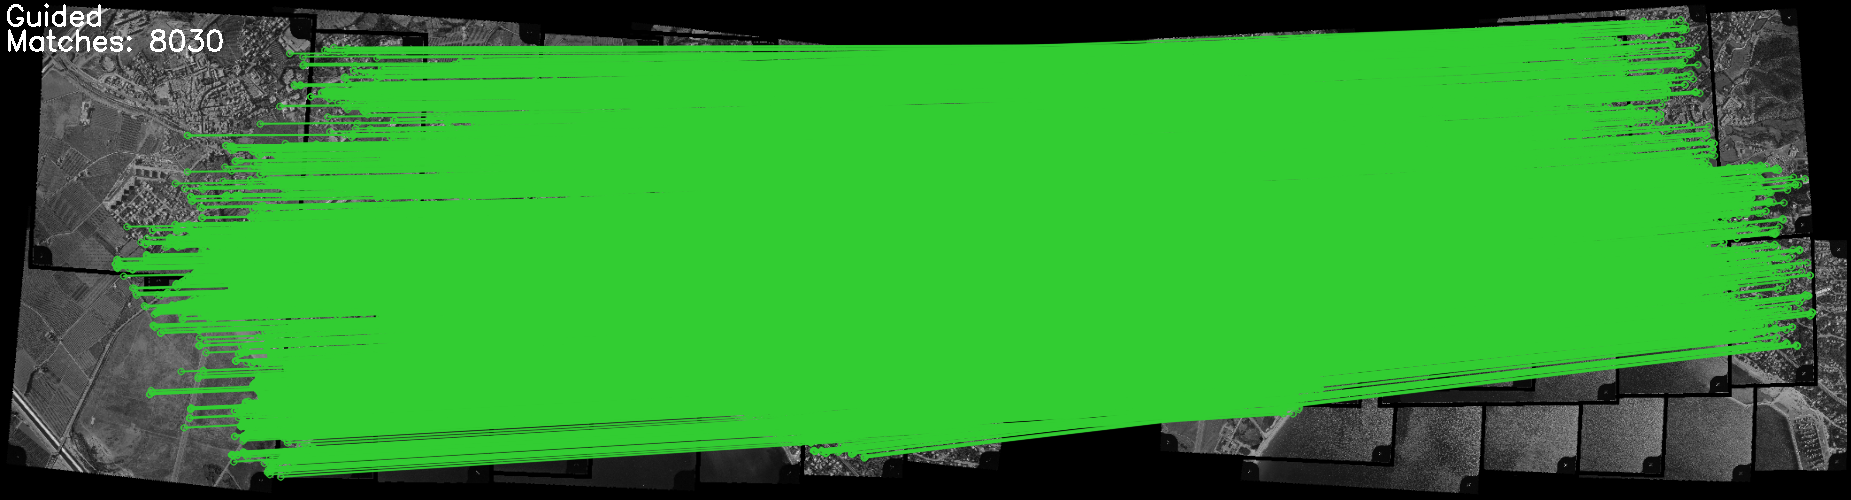
\includegraphics[width=6.8cm]{images/Chapitre4/Precise-SpGDSMHomol-1966-1970-GuidedSIFT-3DRANSAC-CrossCorrelation-PileImg_Ortho-MEC-Malt_Tapas_1966_Ortho-MEC-Malt_Tapas_1970.png}
			\end{minipage}%
		}
		\subfigure[$Patch_{SIFTDSM}$]{
			\begin{minipage}[t]{0.48\linewidth}
				\centering
				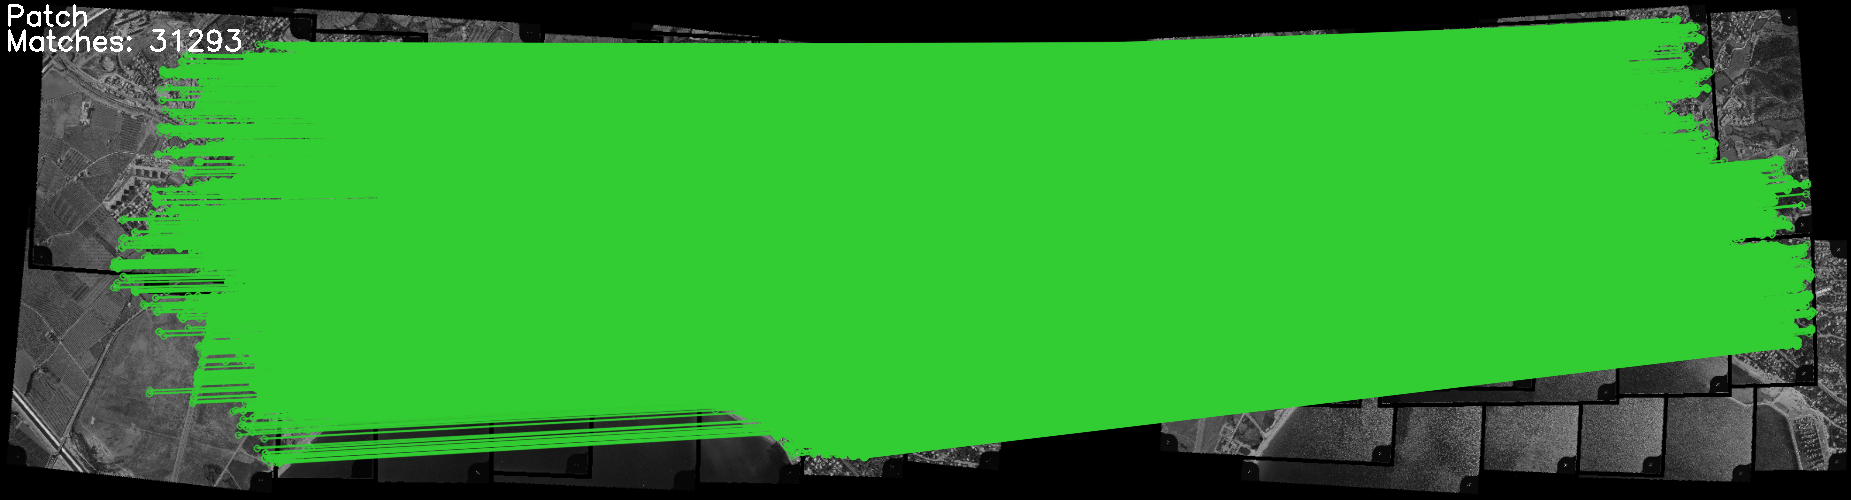
\includegraphics[width=6.8cm]{images/Chapitre4/Precise-SIFTDSMHomol-1966-1970-SuperGlue-3DRANSAC-CrossCorrelation-PileImg_Ortho-MEC-Malt_Tapas_1966_Ortho-MEC-Malt_Tapas_1970.png}
			\end{minipage}%
		}
		\subfigure[$Guided_{SIFTDSM}$]{
			\begin{minipage}[t]{0.48\linewidth}
				\centering
				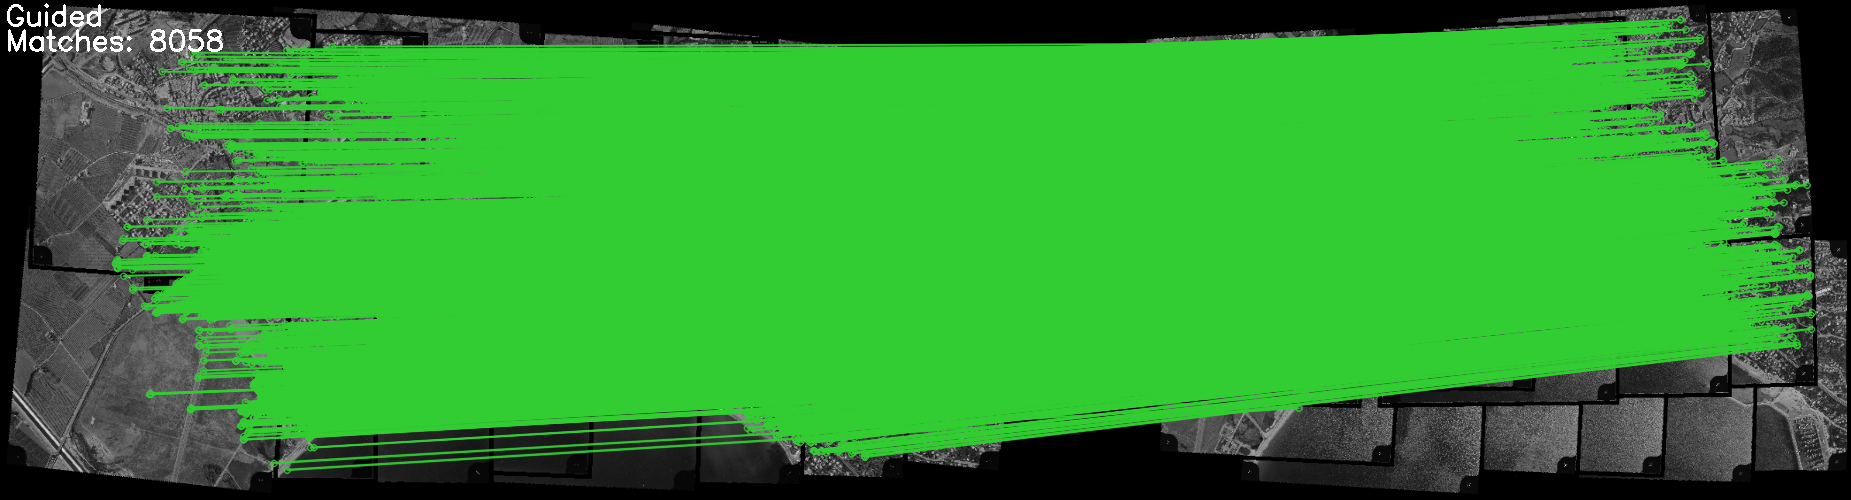
\includegraphics[width=6.8cm]{images/Chapitre4/Precise-SIFTDSMHomol-1966-1970-GuidedSIFT-3DRANSAC-CrossCorrelation-PileImg_Ortho-MEC-Malt_Tapas_1966_Ortho-MEC-Malt_Tapas_1970.png}
			\end{minipage}%
		}
		\caption{Precise matching visualization of \textbf{Fr{\'e}jus 1966 and 1970}. (a) Image pairs to be matched, with red rectangles indicating the common zone. (b) Numbers of tentative, enhanced and final matches recovered with $Patch_{SpGDSM}$, $Guided_{SpGDSM}$, $Patch_{SIFTDSM}$ and $Guided_{SIFTDSM}$ individually. (c-f) Visualization of final matches recovered with $Patch_{SpGDSM}$, $Guided_{SpGDSM}$, $Patch_{SIFTDSM}$ and $Guided_{SIFTDSM}$ individually.}
		\label{MatchVizFrejus1966-1970}
	\end{center}
\end{figure*} 


\begin{figure*}[htbp]
	\begin{center}
		\subfigure[Common zone]{
			\begin{minipage}[t]{0.48\linewidth}
				\centering
				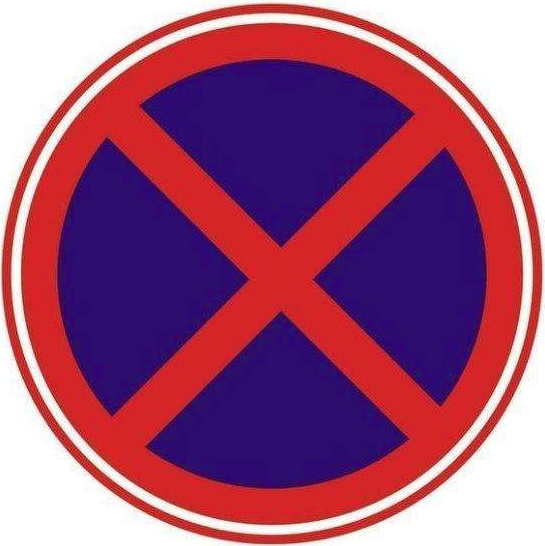
\includegraphics[width=6.8cm]{images/Chapitre4/Pseudo-Ortho-MEC-Malt_Tapas_1954_Ortho-MEC-Malt_Tapas_1966.png}
			\end{minipage}%
		}
		\subfigure[Number of recovered matches]{
			\begin{minipage}[t]{0.48\linewidth}
				\centering
				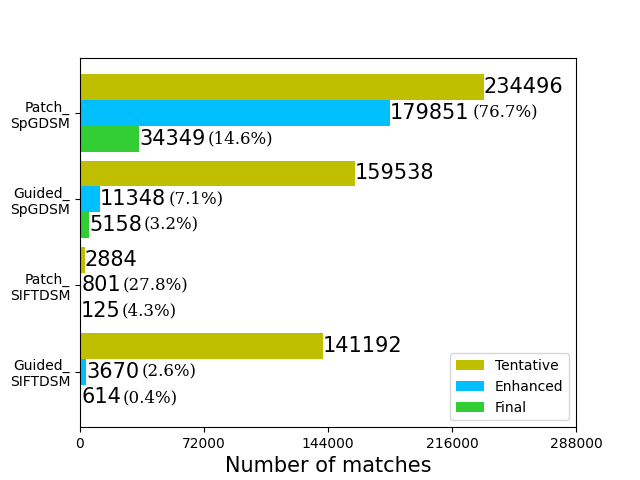
\includegraphics[width=5.8cm]{images/Chapitre4/PlotBarH-Frejus1954-1966.png}
			\end{minipage}%
		}
		\subfigure[$Patch_{SpGDSM}$]{
			\begin{minipage}[t]{0.48\linewidth}
				\centering
				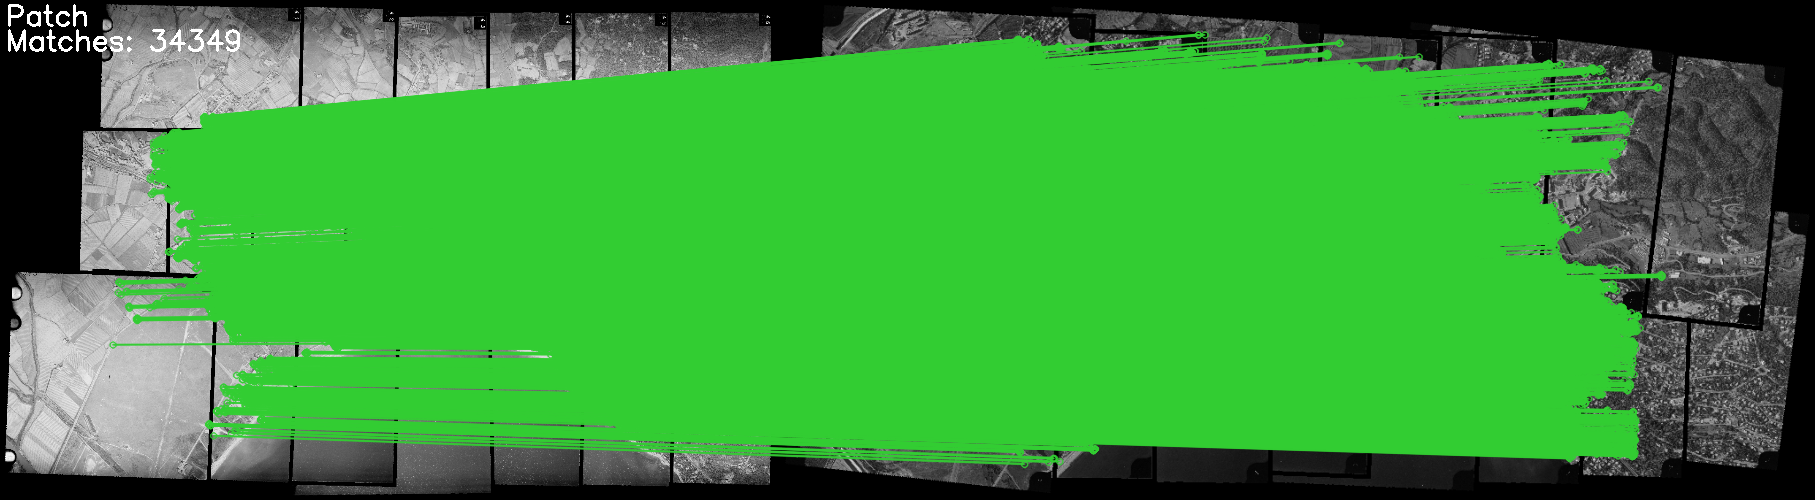
\includegraphics[width=6.8cm]{images/Chapitre4/Precise-SpGDSMHomol-1954-1966-SuperGlue-3DRANSAC-CrossCorrelation-PileImg_Ortho-MEC-Malt_Tapas_1954_Ortho-MEC-Malt_Tapas_1966.png}
			\end{minipage}%
		}
		\subfigure[$Guided_{SpGDSM}$]{
			\begin{minipage}[t]{0.48\linewidth}
				\centering
				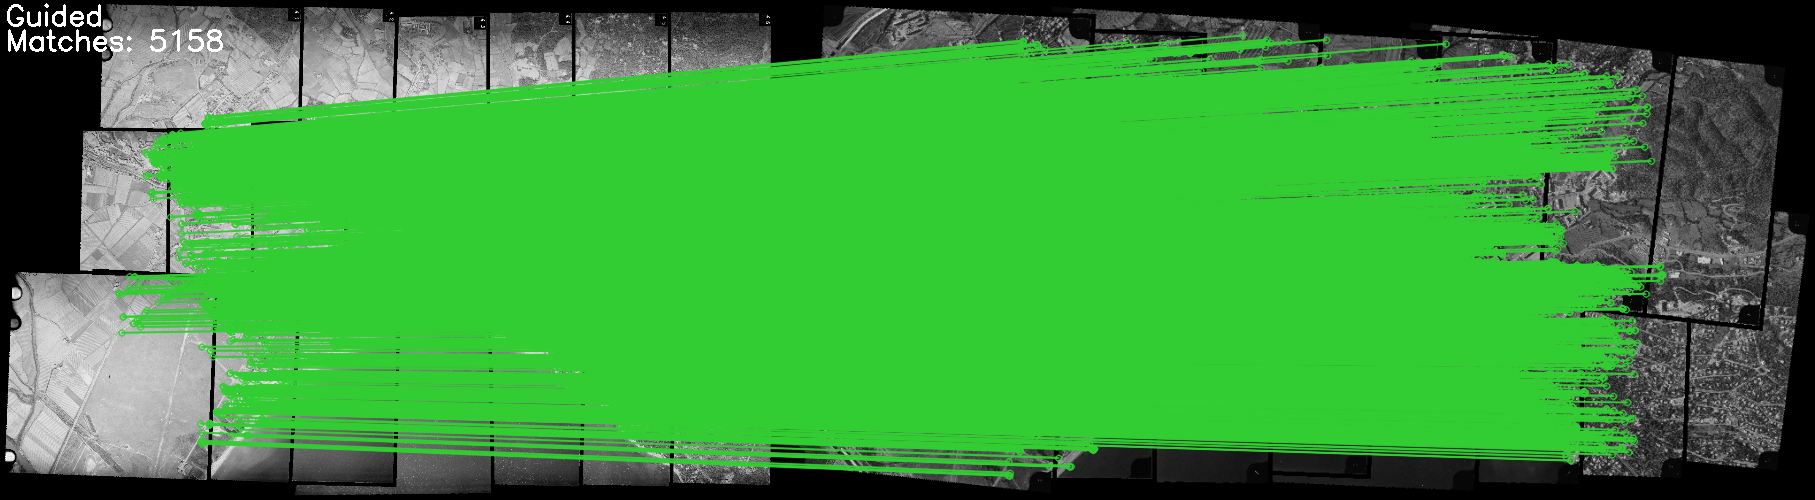
\includegraphics[width=6.8cm]{images/Chapitre4/Precise-SpGDSMHomol-1954-1966-GuidedSIFT-3DRANSAC-CrossCorrelation-PileImg_Ortho-MEC-Malt_Tapas_1954_Ortho-MEC-Malt_Tapas_1966.png}
			\end{minipage}%
		}
		\subfigure[$Patch_{SIFTDSM}$]{
			\begin{minipage}[t]{0.48\linewidth}
				\centering
				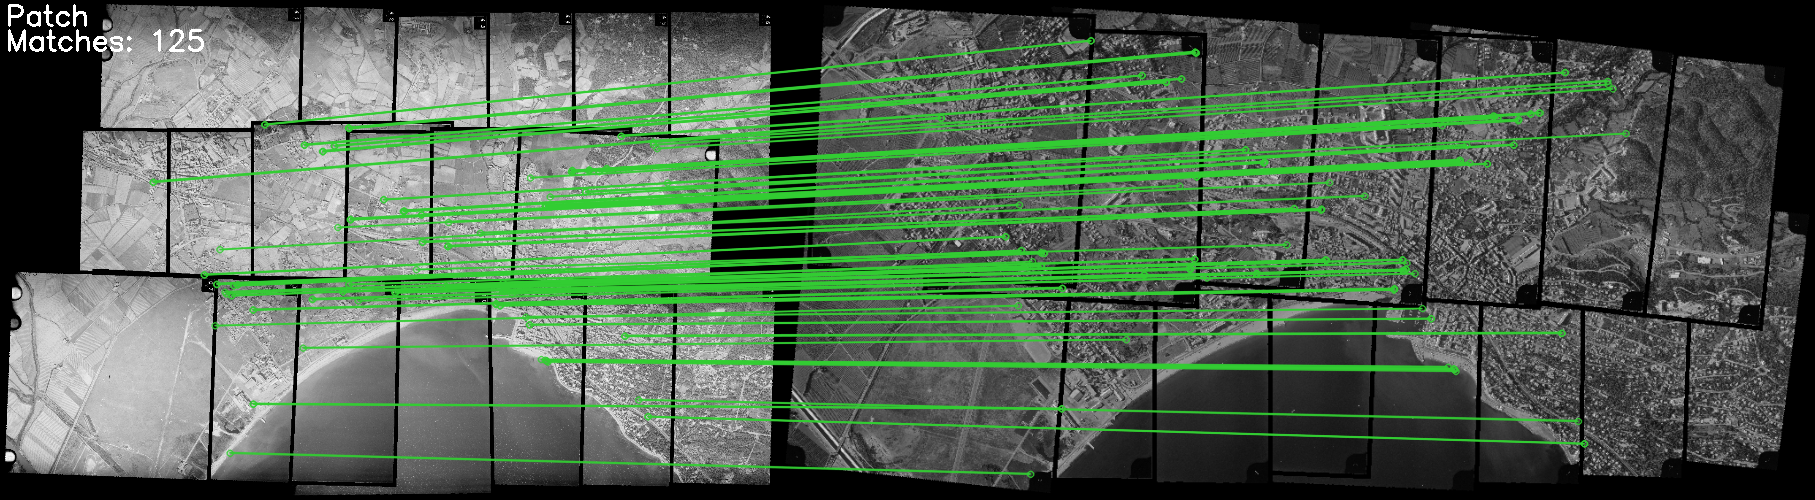
\includegraphics[width=6.8cm]{images/Chapitre4/Precise-SIFTDSMHomol-1954-1966-SuperGlue-3DRANSAC-CrossCorrelation-PileImg_Ortho-MEC-Malt_Tapas_1954_Ortho-MEC-Malt_Tapas_1966.png}
			\end{minipage}%
		}
		\subfigure[$Guided_{SIFTDSM}$]{
			\begin{minipage}[t]{0.48\linewidth}
				\centering
				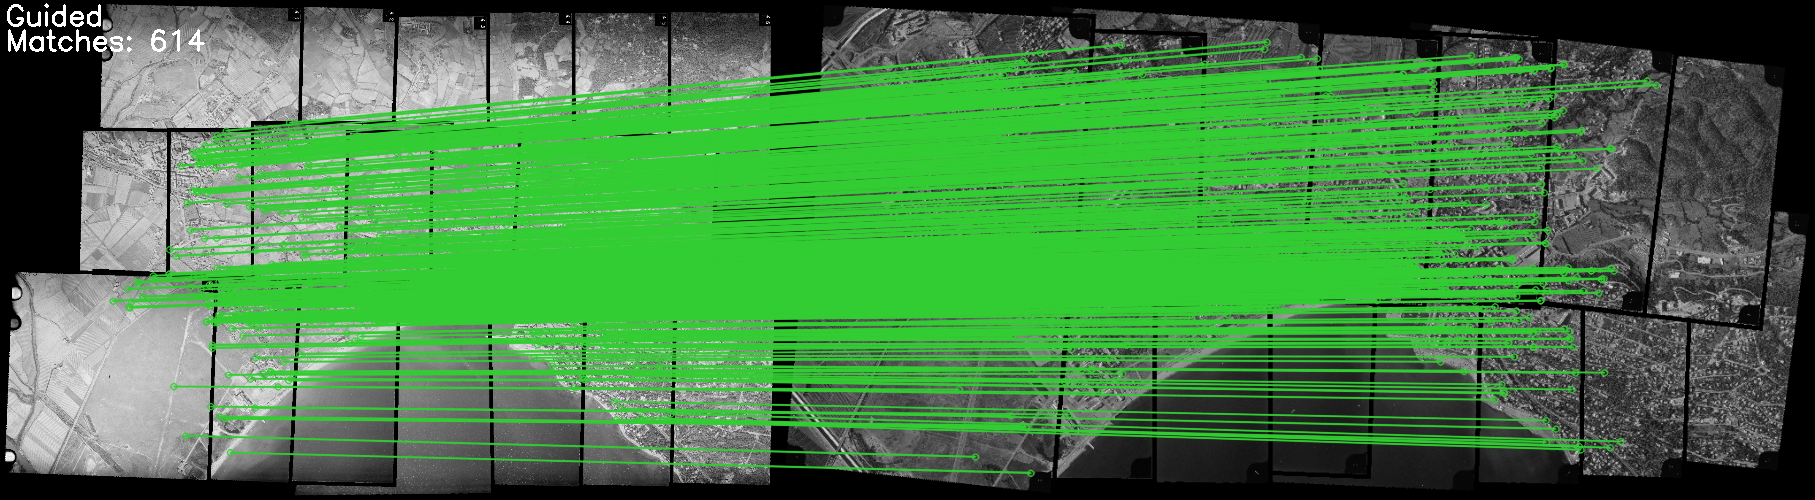
\includegraphics[width=6.8cm]{images/Chapitre4/Precise-SIFTDSMHomol-1954-1966-GuidedSIFT-3DRANSAC-CrossCorrelation-PileImg_Ortho-MEC-Malt_Tapas_1954_Ortho-MEC-Malt_Tapas_1966.png}
			\end{minipage}%
		}
		\caption{Precise matching visualization of \textbf{Fr{\'e}jus 1954 and 1966}. (a) Image pairs to be matched, with red rectangles indicating the common zone. (b) Numbers of tentative, enhanced and final matches recovered with $Patch_{SpGDSM}$, $Guided_{SpGDSM}$, $Patch_{SIFTDSM}$ and $Guided_{SIFTDSM}$ individually. (c-f) Visualization of final matches recovered with $Patch_{SpGDSM}$, $Guided_{SpGDSM}$, $Patch_{SIFTDSM}$ and $Guided_{SIFTDSM}$ individually.}
		\label{MatchVizFrejus1954-1966}
	\end{center}
\end{figure*} 

%%%%%%%%%%%%%%%%%Pezenas
\begin{figure*}[htbp]
	\begin{center}
		\subfigure[Common zone]{
			\begin{minipage}[t]{0.48\linewidth}
				\centering
				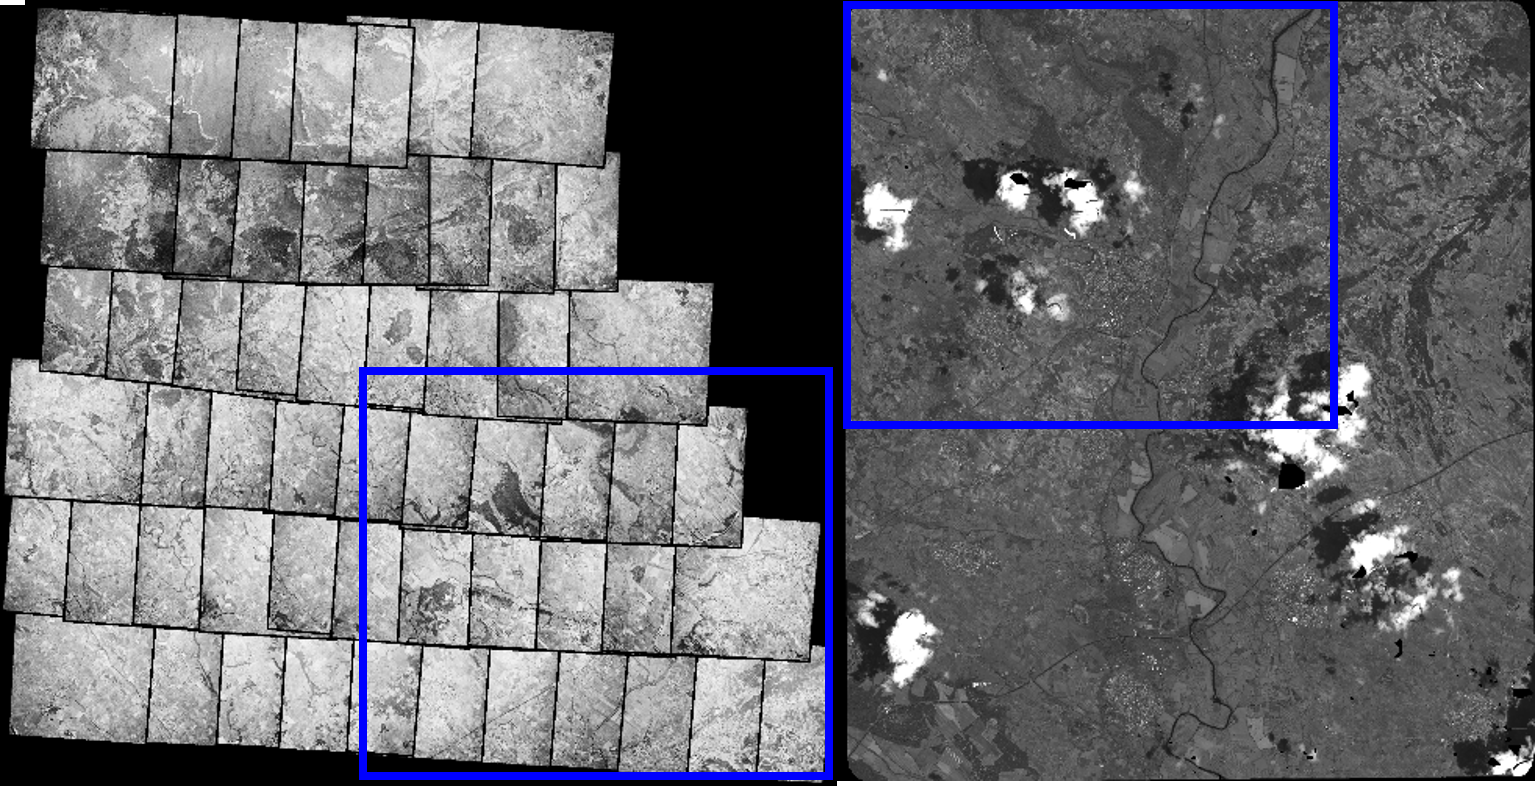
\includegraphics[width=6.8cm]{images/Chapitre4/Pseudo-Ortho-MEC-Malt_Tapas_1971_Ortho-MEC-Malt_Satellite.png}
			\end{minipage}%
		}
		\subfigure[Number of recovered matches]{
			\begin{minipage}[t]{0.48\linewidth}
				\centering
				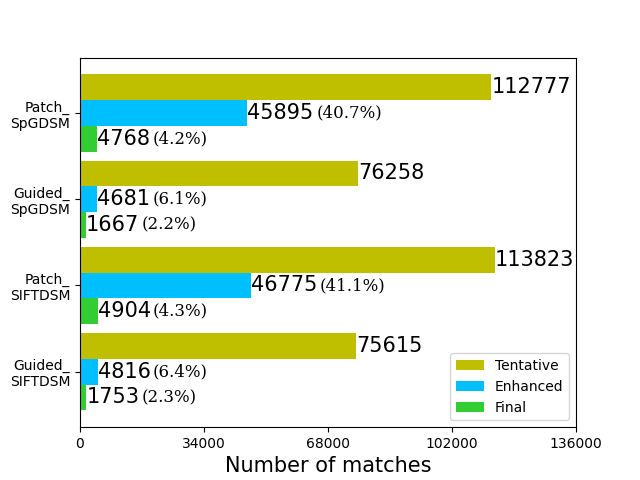
\includegraphics[width=5.8cm]{images/Chapitre4/PlotBarH-Pezenas1971-2014.png}
			\end{minipage}%
		}
		\subfigure[$Patch_{SpGDSM}$]{
			\begin{minipage}[t]{0.48\linewidth}
				\centering
				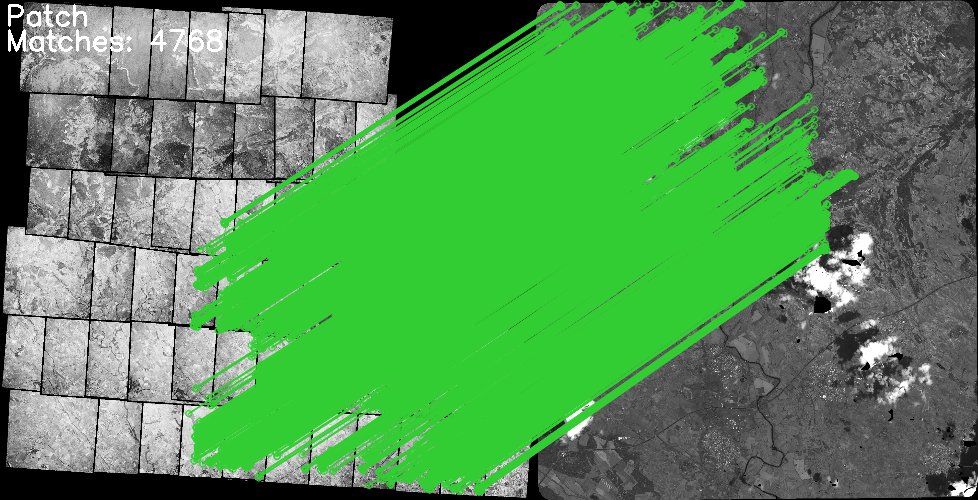
\includegraphics[width=6.8cm]{images/Chapitre4/Precise-SpGDSMHomol-SuperGlue-3DRANSAC-CrossCorrelation-PileImg_Ortho-MEC-Malt_Tapas_1971_Ortho-MEC-Malt_Satellite.png}
			\end{minipage}%
		}
		\subfigure[$Guided_{SpGDSM}$]{
			\begin{minipage}[t]{0.48\linewidth}
				\centering
				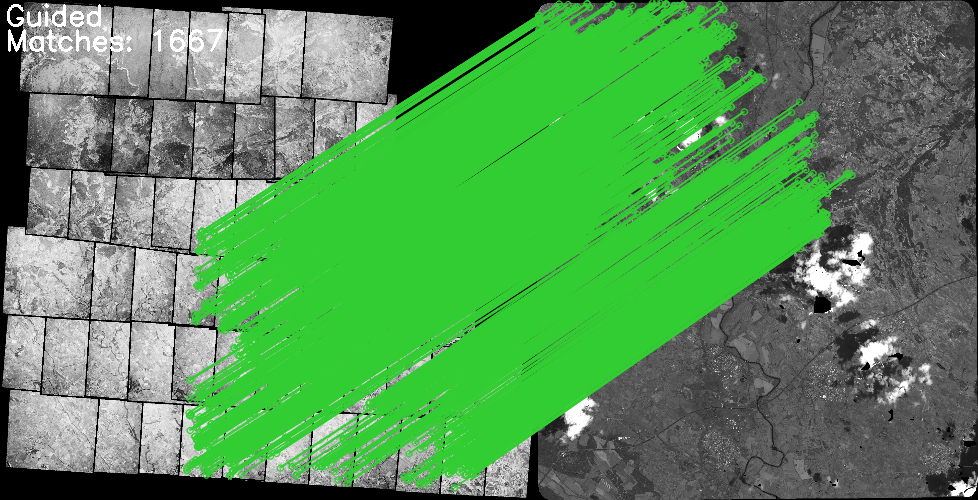
\includegraphics[width=6.8cm]{images/Chapitre4/Precise-SpGDSMHomol-GuidedSIFT-3DRANSAC-CrossCorrelation-PileImg_Ortho-MEC-Malt_Tapas_1971_Ortho-MEC-Malt_Satellite.png}
			\end{minipage}%
		}
		\subfigure[$Patch_{SIFTDSM}$]{
			\begin{minipage}[t]{0.48\linewidth}
				\centering
				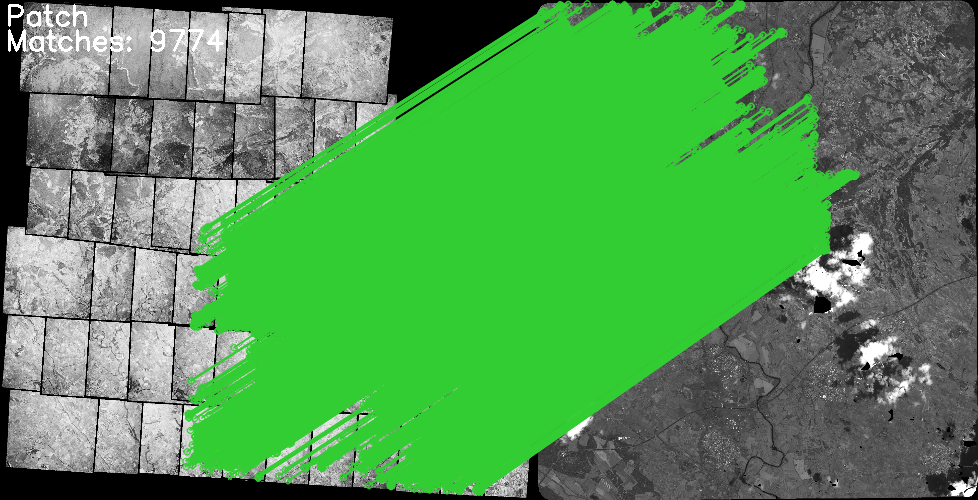
\includegraphics[width=6.8cm]{images/Chapitre4/Precise-SIFTDSMHomol-SuperGlue-3DRANSAC-CrossCorrelation-PileImg_Ortho-MEC-Malt_Tapas_1971_Ortho-MEC-Malt_Satellite.png}
			\end{minipage}%
		}
		\subfigure[$Guided_{SIFTDSM}$]{
			\begin{minipage}[t]{0.48\linewidth}
				\centering
				\includegraphics[width=6.8cm]{images/Chapitre4/Precise-SIFTDSMHomol-GuidedSIFT-3DRANSAC-CrossCorrelation-PileImg_Ortho-MEC-Malt_Tapas_1971_Ortho-MEC-Malt_Satellite.png}
			\end{minipage}%
		}
		\caption{Precise matching visualization of \textbf{Pezenas 1971 and 2014 (Satellite)}. (a) Image pairs to be matched, with red rectangles indicating the common zone. (b) Numbers of tentative, enhanced and final matches recovered with $Patch_{SpGDSM}$, $Guided_{SpGDSM}$, $Patch_{SIFTDSM}$ and $Guided_{SIFTDSM}$ individually. (c-f) Visualization of final matches recovered with $Patch_{SpGDSM}$, $Guided_{SpGDSM}$, $Patch_{SIFTDSM}$ and $Guided_{SIFTDSM}$ individually.}
		\label{MatchVizPezenas}
	\end{center}
\end{figure*} 

%Pseudo-Ortho-MEC-Malt_Tapas_1991_Ortho-MEC-Malt_Tapas_1994

\begin{figure*}[htbp]
	\begin{center}
		\subfigure[Common zone]{
			\begin{minipage}[t]{0.48\linewidth}
				\centering
				\includegraphics[width=3.8cm,angle=90]{images/Chapitre3/Pseudo-Ortho-MEC-Malt_Tapas_1991_Ortho-MEC-Malt_Tapas_1994.png}
			\end{minipage}%
		}
		\subfigure[Number of recovered matches]{
			\begin{minipage}[t]{0.48\linewidth}
				\centering
				\includegraphics[width=5.8cm]{images/Chapitre4/PlotBarH-Kobe1991-1995.png}
			\end{minipage}%
		}
		\subfigure[$Patch_{SpGDSM}$]{
			\begin{minipage}[t]{0.48\linewidth}
				\centering
				\includegraphics[width=3.8cm,angle=90]{images/Chapitre4/Precise-SpGDSMHomol-SuperGlue-3DRANSAC-CrossCorrelation-PileImg_Ortho-MEC-Malt_Tapas_1991_Ortho-MEC-Malt_Tapas_1994.png}
			\end{minipage}%
		}
		\subfigure[$Guided_{SpGDSM}$]{
			\begin{minipage}[t]{0.48\linewidth}
				\centering
				\includegraphics[width=3.8cm,angle=90]{images/Chapitre4/Precise-SpGDSMHomol-GuidedSIFT-3DRANSAC-CrossCorrelation-PileImg_Ortho-MEC-Malt_Tapas_1991_Ortho-MEC-Malt_Tapas_1994.png}
			\end{minipage}%
		}
		\subfigure[$Patch_{SIFTDSM}$]{
			\begin{minipage}[t]{0.48\linewidth}
				\centering
				\includegraphics[width=3.8cm,angle=90]{images/Chapitre4/Precise-SIFTDSMHomol-SuperGlue-3DRANSAC-CrossCorrelation-PileImg_Ortho-MEC-Malt_Tapas_1991_Ortho-MEC-Malt_Tapas_1994.png}
			\end{minipage}%
		}
		\subfigure[$Guided_{SIFTDSM}$]{
			\begin{minipage}[t]{0.48\linewidth}
				\centering
				\includegraphics[width=3.8cm,angle=90]{images/Chapitre4/Precise-SIFTDSMHomol-GuidedSIFT-3DRANSAC-CrossCorrelation-PileImg_Ortho-MEC-Malt_Tapas_1991_Ortho-MEC-Malt_Tapas_1994.png}
			\end{minipage}%
		}
		\caption{Precise matching visualization of \textbf{Kobe 1991 and 1995}. (a) Image pairs to be matched, with red rectangles indicating the common zone. (b) Numbers of tentative, enhanced and final matches recovered with $Patch_{SpGDSM}$, $Guided_{SpGDSM}$, $Patch_{SIFTDSM}$ and $Guided_{SIFTDSM}$ individually. (c-f) Visualization of final matches recovered with $Patch_{SpGDSM}$, $Guided_{SpGDSM}$, $Patch_{SIFTDSM}$ and $Guided_{SIFTDSM}$ individually.}
		\label{MatchVizKobe}
	\end{center}
\end{figure*} 

\subsubsection{DoD}


\begin{figure*}[htbp]
	\begin{center}
		\subfigure[\ac{DoD}$_{Pezenas1971}^{Patch_{SpGDSM}}$]{
			\begin{minipage}[t]{0.31\linewidth}
				\centering
				%\includegraphics[width=4.5cm,trim=680 80 50 230,clip]{images/Chapitre4/DoD1971Ortho-SuperGlue-Satellite.png}
				\includegraphics[width=4.5cm,trim=840 70 290 340,clip]{images/Chapitre4/DoD1971_Patch_SpGDSM.png}
			\end{minipage}%
		}
		\subfigure[\ac{DoD}$_{Pezenas1971}^{Guided_{SpGDSM}}$]{
			\begin{minipage}[t]{0.31\linewidth}
				\centering
				\includegraphics[width=4.5cm,trim=840 70 290 340,clip]{images/Chapitre4/DoD1971_Guided_SpGDSM.png}
			\end{minipage}%
		}\\
		
		\subfigure[\ac{DoD}$_{Pezenas1971}^{Patch_{SIFTDSM}}$]{
			\begin{minipage}[t]{0.31\linewidth}
				\centering
				\includegraphics[width=4.5cm,trim=840 70 290 340,clip]{images/Chapitre4/DoD1971_Patch_SIFTDSM.png}
			\end{minipage}%
		}
		\subfigure[\ac{DoD}$_{Pezenas1971}^{Guided_{SIFTDSM}}$]{
			\begin{minipage}[t]{0.31\linewidth}
				\centering
				\includegraphics[width=4.5cm,trim=840 70 290 340,clip]{images/Chapitre4/DoD1971_Guided_SIFTDSM.png}
			\end{minipage}%
		}\\
		
		
		\subfigure[\ac{DoD} legend]{
			\begin{minipage}[t]{1\linewidth}
				\centering
				\includegraphics[width=11cm]{images/Chapitre4/LegendDoD.png}
			\end{minipage}%
		}
		\caption{{\scriptsize \ac{DoD}s between free epoch \textbf{Pezenas 1971, 1981} and reference satellite epoch \textbf{2014} with methods $SuperGlue_{Ortho}$ (a, e), $SuperGlue_{DSM}$ (b, f), $SIFT_{Ortho}$ (c, g) and $SIFT_{DSM}$ (d, h). The holes among them are areas covered with clouds which are masked out. The prohibition sign means the corresponding method failed.}}
		\label{DoDPezenas-Satellite}
	\end{center}
\end{figure*} 

\begin{table}%[H]
	\footnotesize
	\centering
	\begin{tabular}{||l|l|c|c|c||}\hline
		& &$\mu$ [m]&$\sigma$ [m]&$|\mu|$ [m]\\\hline\hline
%		\multirow{6}{*}{$DoD^{Frejus}_{1954-2014}$}
%		&${SuperGlue_{ImgPairs}}$ & 5.70 & 6.32 & 6.62\\
%		&${SuperGlue_{Ortho}}$ & 2.19 & 6.46 & 4.55\\
%		&${SuperGlue_{DSM}}$ & 2.07 & 4.87 & \textbf{3.83} \\
%		&${SIFT_{ImgPairs}}$ & / & / & / \\
%		&${SIFT_{Ortho}}$ & / & / & / \\
%		&${SIFT_{DSM}}$ & 6.92 & 8.47 & 8.04\\\hline
%		
%		\multirow{6}{*}{$DoD^{Frejus}_{1966-2014}$}
%		&${SuperGlue_{ImgPairs}}$ & -1.36 & 3.82 & 2.90\\
%		&${SuperGlue_{Ortho}}$ & -0.37 & 4.22 & 3.01\\
%		&${SuperGlue_{DSM}}$ & -0.46 & 3.77 & \textbf{2.68}\\
%		&${SIFT_{ImgPairs}}$ & / & / & / \\
%		&${SIFT_{Ortho}}$ & / & / & / \\
%		&${SIFT_{DSM}}$ & -1.72 & 4.92 & 3.75\\\hline
%		
%		\multirow{6}{*}{$DoD^{Frejus}_{1970-2014}$}
%		&${SuperGlue_{ImgPairs}}$ & -5.04 & 5.09 & 5.70\\
%		&${SuperGlue_{Ortho}}$ & -2.63 & 5.18 & \textbf{4.39}\\
%		&${SuperGlue_{DSM}}$ & -1.71 & 5.75 & 4.61\\
%		&${SIFT_{ImgPairs}}$ & / & / & / \\
%		&${SIFT_{Ortho}}$ & / & / & / \\
%		&${SIFT_{DSM}}$ & -3.17 & 5.44 & 4.71\\\hline
		
		%%%%%%%%%%%%%%%%%%%%%%%%satellite
		\multirow{4}{*}{$DoD^{Pezenas}_{1971-2014(Satellite)}$}
&${Patch_{SpGDSM}}$ & -0.34 & 4.39 & 2.28\\
&${Guided_{SpGDSM}}$ & -0.65 & 4.46 & 2.45\\
&${Patch_{SIFTDSM}}$ & -0.49 & 4.41 & 2.29\\
&${Guided_{SIFTDSM}}$ & -0.57 & 4.38 & \textbf{2.27}\\\hline


%		\multirow{4}{*}{$DoD^{Pezenas}_{1971-2014(Satellite)}$}
%		%&${SuperGlue_{DSM}}$ & -3.70 & 10.65 & 8.29\\
%		&${Patch_{SpGDSM}}$ & -0.45 & 4.62 & 2.34\\
%		&${Guided_{SpGDSM}}$ & -0.61 & 4.75 & 2.47\\
%		%&${SIFT_{DSM}}$ & -0.68 & 8.11 & 5.80 \\
%		&${Patch_{SIFTDSM}}$ & -0.35 & 4.70 & \textbf{2.28}\\
%		&${Guided_{SIFTDSM}}$ & -0.48 & 4.39 & 2.33\\\hline
				
%		&${SuperGlue_{Ortho}}$ & / & / & /\\
%		&${SuperGlue_{DSM}}$ & -3.70 & 10.65 & 8.29\\
%		%&${SuperGlue_{DSM}}$ & -1.85 & 13.24 & 9.15\\
%		&${SIFT_{Ortho}}$ & / & / & /\\
%		&${SIFT_{DSM}}$ & -0.68 & 8.11 & \textbf{5.80} \\\hline
%		%&${SIFT_{DSM}}$ & 0.58 & 7.82 & \textbf{3.18}\\\hline
		
		\multirow{6}{*}{$DoD^{Kobe}_{1991-1995}$}
		&${Patch_{SpGDSM}}$ & 1.93 & 10.26 & 3.99\\
		&${Guided_{SpGDSM}}$ & 2.03 & 11.74 & 4.30\\
		&${Patch_{SIFTDSM}}$ & 1.80 & 10.36 & 4.00\\
		&${Guided_{SIFTDSM}}$ & 1.84 & 9.48 & \textbf{3.87}\\

%		&${SuperGlue_{ImgPairs}}$ & -1.63 & 13.85 & \textbf{7.24}\\
%		%&${SIFT_{ImgPairs}}$ & 167.46 & 121.26 & 168.47\\
%		&${SuperGlue_{Ortho}}$ & -0.54 & 14.83 & 7.78\\
%		%&${SIFT_{Ortho}}$ & 4.29 & 41.89 & 26.01\\
%		&${SuperGlue_{DSM}}$ & -0.75 & 14.62 & 7.95\\
%		&${SIFT_{ImgPairs}}$ & / & / & / \\
%		&${SIFT_{Ortho}}$ & / & / & / \\
%		&${SIFT_{DSM}}$ & 0.27 & 14.40 & 7.57\\\hline
		
	\end{tabular}
	\caption{Average value $\mu$, standard deviation $\sigma$, and absolute average value $|\mu|$ of all the \ac{DoD}s in Figure~\ref{DoDFrejus}, ~\ref{DoDPezenas}, ~\ref{DoDPezenas-Satellite} and ~\ref{DoDKobe}.}
	\label{DoDStatistic}
\end{table}

\subsubsection{Ground displacement}

\section{Conclusion}

\section{Discussion}
